%%%%%%%%%%%%%%%%%%%%%%%%%%%%%%%%%%%%%%%%%
% kaobook
% LaTeX Template
% Version 1.3 (December 9, 2021)
%
% This template originates from:
% https://www.LaTeXTemplates.com
%
% For the latest template development version and to make contributions:
% https://github.com/fmarotta/kaobook
%
% Authors:
% Federico Marotta (federicomarotta@mail.com)
% Based on the doctoral thesis of Ken Arroyo Ohori (https://3d.bk.tudelft.nl/ken/en)
% and on the Tufte-LaTeX class.
% Modified for LaTeX Templates by Vel (vel@latextemplates.com)
%
% License:
% CC0 1.0 Universal (see included MANIFEST.md file)
%
%%%%%%%%%%%%%%%%%%%%%%%%%%%%%%%%%%%%%%%%%

\documentclass[
	a4paper, % Page size
	fontsize=9pt, % Base font size
	twoside=true, % Use different layouts for even and odd pages (in particular, if twoside=true, the margin column will be always on the outside)
	%open=any, % If twoside=true, uncomment this to force new chapters to start on any page, not only on right (odd) pages
	%chapterentrydots=true, % Uncomment to output dots from the chapter name to the page number in the table of contents
	numbers=noenddot, % Comment to output dots after chapter numbers; the most common values for this option are: enddot, noenddot and auto (see the KOMAScript documentation for an in-depth explanation)
]{kaobook}

% Choose the language
\ifxetexorluatex
	\usepackage{polyglossia}
	\setmainlanguage{english}
\else
	\usepackage[english]{babel} % Load characters and hyphenation
\fi
\usepackage[english=british]{csquotes}	% English quotes


\usepackage{svg}
\usepackage{outlines}
% Load packages for testing
\usepackage{blindtext}
\usepackage{booktabs}
\usepackage{amsmath}
\usepackage{amssymb}
% \usepackage{showframe} % Uncomment to show boxes around the text area, margin, header and footer
%\usepackage{showlabels} % Uncomment to output the content of \label commands to the document where they are used

% Load the bibliography package
\usepackage{kaobiblio}
\usepackage{lipsum}
\usepackage{todonotes}

\addbibresource{EV.bib} % Bibliography file
\addbibresource{ev-old.bib} % Bibliography file
\addbibresource{Matsim.bib} % Bibliography file

% Load mathematical packages for theorems and related environments
\usepackage[framed=true]{kaotheorems}

% Load the package for hyperreferences
\usepackage{kaorefs}

\graphicspath{{examples/documentation/images/}{images/}} % Paths in which to look for images

\makeindex[columns=3, title=Alphabetical Index, intoc] % Make LaTeX produce the files required to compile the index

\makeglossaries % Make LaTeX produce the files required to compile the glossary
\newacronym{EV}{EV}{electric vehicle}
\newacronym{ICE}{ICE}{internal combustion engine vehicle}
\newacronym{CS}{CS}{charging station}
\newacronym{CP}{CD}{charging point}
\newacronym{POI}{CD}{point of interest}
\newacronym{CD}{CD}{charging demand}
\newacronym{EU}{EU}{European Union}
\newacronym{GAN}{GAN}{generative adversarial network}
\newacronym{NN}{NN}{neural network}
\newacronym{ML}{ML}{machine learning}
\newacronym{ZSJ}{ZSJ}{basic settlement unit (základní sídelní jednotka)}
\newacronym{TSK}{TSK}{Technical Administration of Communications of the City of Prague, a.s. (Technická správa komunikací hlavního města Prahy, a.s.)}
\newacronym{ABM}{ABM}{Agent based model}
\newacronym{VAE}{VAE}{variational autoencoder}
 % Include the glossary definitions

\makenomenclature % Make LaTeX produce the files required to compile the nomenclature

% Reset sidenote counter at chapters
%\counterwithin*{sidenote}{chapter}

%----------------------------------------------------------------------------------------

\begin{document}

%----------------------------------------------------------------------------------------
%	BOOK INFORMATION
%----------------------------------------------------------------------------------------

\titlehead{CTU FEL Prague}
\subject{Master thesis}

\title[huh]{EV vehicles}
\subtitle{and charging demand}

\author[Bc. Jakub Zíka]{Bc. Jakub Zíka}

% \date{\today}

\publishers{CTU FEL}

%----------------------------------------------------------------------------------------

\frontmatter % Denotes the start of the pre-document content, uses roman numerals

%----------------------------------------------------------------------------------------
%	OPENING PAGE
%----------------------------------------------------------------------------------------

%\makeatletter
%\extratitle{
%	% In the title page, the title is vspaced by 9.5\baselineskip
%	\vspace*{9\baselineskip}
%	\vspace*{\parskip}
%	\begin{center}
%		% In the title page, \huge is set after the komafont for title
%		\usekomafont{title}\huge\@title
%	\end{center}
%}
%\makeatother

%----------------------------------------------------------------------------------------
%	COPYRIGHT PAGE
%----------------------------------------------------------------------------------------

\makeatletter
\uppertitleback{\@titlehead} % Header

\lowertitleback{
	\textbf{Disclaimer}\\
	You can edit this page to suit your needs. For instance, here we have a no copyright statement, a colophon and some other information. This page is based on the corresponding page of Ken Arroyo Ohori's thesis, with minimal changes.

	\medskip

	\textbf{No copyright}\\
	\cczero\ This book is released into the public domain using the CC0 code. To the extent possible under law, I waive all copyright and related or neighbouring rights to this work.

	To view a copy of the CC0 code, visit: \\\url{http://creativecommons.org/publicdomain/zero/1.0/}

	\medskip

	\textbf{Colophon} \\
	This document was typeset with the help of \href{https://sourceforge.net/projects/koma-script/}{\KOMAScript} and \href{https://www.latex-project.org/}{\LaTeX} using the \href{https://github.com/fmarotta/kaobook/}{kaobook} class.

	The source code of this book is available at:\\\url{https://github.com/fmarotta/kaobook}

	(You are welcome to contribute!)

	\medskip

	\textbf{Publisher} \\
	First printed in May 2019 by \@publishers
}
\makeatother

%----------------------------------------------------------------------------------------
%	DEDICATION
%----------------------------------------------------------------------------------------	

%----------------------------------------------------------------------------------------
%	OUTPUT TITLE PAGE AND PREVIOUS
%----------------------------------------------------------------------------------------

% Note that \maketitle outputs the pages before here

\maketitle

%----------------------------------------------------------------------------------------
%	PREFACE
%----------------------------------------------------------------------------------------

% \chapter*{Preface}
\addcontentsline{toc}{chapter}{Preface} % Add the preface to the table of contents as a chapter

I am of the opinion that every \LaTeX\xspace geek, at least once during 
his life, feels the need to create his or her own class: this is what 
happened to me and here is the result, which, however, should be seen as 
a work still in progress. Actually, this class is not completely 
original, but it is a blend of all the best ideas that I have found in a 
number of guides, tutorials, blogs and tex.stackexchange.com posts. In 
particular, the main ideas come from two sources:

\begin{itemize}
	\item \href{https://3d.bk.tudelft.nl/ken/en/}{Ken Arroyo Ohori}'s 
	\href{https://3d.bk.tudelft.nl/ken/en/nl/ken/en/2016/04/17/a-1.5-column-layout-in-latex.html}{Doctoral 
	Thesis}, which served, with the author's permission, as a backbone 
	for the implementation of this class;
	\item The 
		\href{https://github.com/Tufte-LaTeX/tufte-latex}{Tufte-Latex 
			Class}, which was a model for the style.
\end{itemize}

The first chapter of this book is introductory and covers the most
essential features of the class. Next, there is a bunch of chapters 
devoted to all the commands and environments that you may use in writing 
a book; in particular, it will be explained how to add notes, figures 
and tables, and references. The second part deals with the page layout 
and design, as well as additional features like coloured boxes and 
theorem environments.

I started writing this class as an experiment, and as such it should be 
regarded. Since it has always been intended for my personal use, it may
not be perfect but I find it quite satisfactory for the use I want to 
make of it. I share this work in the hope that someone might find here 
the inspiration for writing his or her own class.

\begin{flushright}
	\textit{Federico Marotta}
\end{flushright}

\index{preface}


\begingroup
\tableofcontents % Output the table of contents
\endgroup

%----------------------------------------------------------------------------------------
%	MAIN BODY
%----------------------------------------------------------------------------------------

\mainmatter % Denotes the start of the main document content, resets page numbering and uses arabic numbers
\setchapterstyle{kao} % Choose the default chapter heading style
\pagelayout{wide}
\chapter*{Introduction\;}
\labch{intro}

The invention of the automobile in the late 19th century revolutionized human mobility, enabling unprecedented freedom to traverse long distances. However, this breakthrough hinged not only on the internal combustion engine (ICE) itself but also on the parallel development of a critical support system: gasoline stations. Just as early motorists relied on scattered gas stations to power their journeys, the rise of ICE vehicles necessitated a standardized, accessible network of refueling infrastructure to sustain their adoption. This  relationship between vehicles and their energy infrastructure became a cornerstone of modern transportation, shaping urban planning, economic systems, and global energy policies.


Today, as societies pivot toward sustainability, \acrlongpl{EV} are heralding a similar paradigm shift. Yet their widespread adoption faces a challenge mirroring the early days of automobiles: the need for reliable and efficient charging infrastructure. While \acrlongpl{EV} eliminate tailpipe emissions, their practicality depends on overcoming "range anxiety" and ensuring charging availability aligns with user behavior—issues that gas stations largely resolved for ICE vehicles over a century of iteration. Predicting EV charger usage, therefore, is not merely a technical exercise but a good step in designing infrastructure that mirrors the ubiquity and convenience of gas stations. And helps smoothen transition.

\pagelayout{margin} % Restore margins

\setchapterstyle{kao}
\setchapterpreamble[u]{\margintoc}
\chapter{Motivation - Electromobility and Climate Change}

This chapter explores the fundamental motivations behind the transition to electric mobility, examining the environmental imperatives driving this shift, the evolution of electric vehicles, regulatory frameworks accelerating adoption, and the critical infrastructure challenges that must be addressed to enable widespread electrification of transportation.

\section{Climate change}

Climate change represents one of the most pressing global challenges of our time, with transportation being a significant contributor to greenhouse gas emissions. The Intergovernmental Panel on Climate Change (IPCC) has consistently identified the burning of fossil fuels as the primary driver of anthropogenic climate change, with transportation accounting for approximately 24\% of direct CO\textsubscript{2} emissions from fuel combustion globally \cite{ipcc2022}. Within this sector, road vehicles—particularly those powered by internal combustion engines (ICEs)—are responsible for nearly three-quarters of transport emissions.

The environmental impact of ICE vehicles extends beyond carbon dioxide emissions. These vehicles also produce nitrogen oxides (NO\textsubscript{x}), particulate matter, and other pollutants that contribute to poor air quality, respiratory diseases, and premature deaths in urban areas. The World Health Organization estimates that air pollution causes approximately 7 million premature deaths annually, with vehicle emissions being a significant contributor in urban environments \cite{who2021}.

\begin{figure}[h]
    \centering
    % This is a placeholder for a pie chart showing emission sources
    % \includegraphics[width=0.7\textwidth]{images/emissions-pie-chart.png}
    \caption{Global greenhouse gas emissions by sector, highlighting transportation's contribution (Source: IPCC AR6, 2022)}
    \label{fig:emissions-chart}
\end{figure}

While the scientific consensus on anthropogenic climate change is robust, it is worth acknowledging that the transition to electric mobility is not without controversy. Critics point to the environmental impact of battery production, concerns about electricity generation sources, and the socioeconomic implications of rapid technological change. However, lifecycle analyses consistently demonstrate that even when accounting for battery production and electricity generation, electric vehicles produce significantly lower lifetime emissions than their ICE counterparts in most regions of the world, with this advantage growing as electricity grids incorporate more renewable energy sources \cite{eea2018}.

The climate imperative is particularly challenging for developing nations, which face the dual pressures of reducing emissions while supporting economic growth and mobility needs. These countries often lack the infrastructure and financial resources to rapidly transition to electric mobility, yet they are frequently among the most vulnerable to climate change impacts. International cooperation, technology transfer, and equitable financing mechanisms will be essential to ensure that the global transition to sustainable transportation does not exacerbate existing inequalities.

\section{Electric vehicles}

The history of electric vehicles (EVs) is marked by a fascinating parallel development alongside internal combustion engine vehicles, rather than being a purely modern innovation. In fact, electric vehicles were among the first automobiles developed in the late 19th century, with inventors like Thomas Parker creating practical electric cars as early as 1884. During the early automotive era, electric vehicles competed directly with steam and gasoline-powered vehicles, and were particularly popular in urban environments due to their quiet operation, absence of exhaust, and ease of use compared to early ICE vehicles that required hand-cranking to start.

However, the limitations of early battery technology—particularly in terms of energy density, range, and recharging infrastructure—combined with the discovery of abundant petroleum reserves and the introduction of the electric starter for gasoline engines, led to the dominance of ICE vehicles throughout most of the 20th century. Electric vehicles remained largely confined to specialized applications such as forklifts, golf carts, and other short-range utility vehicles.

The modern resurgence of electric vehicles began in earnest in the late 1990s and early 2000s, driven by advances in lithium-ion battery technology, growing environmental concerns, and regulatory pressures. The introduction of hybrid vehicles like the Toyota Prius served as a transitional technology, familiarizing consumers with electric drivetrains while alleviating range anxiety through the backup of a gasoline engine. The launch of the Tesla Roadster in 2008 demonstrated that electric vehicles could offer performance comparable to or exceeding that of high-end sports cars, challenging perceptions that EVs were inherently limited in capability.

Today's electric vehicles have largely overcome many of the historical limitations that hindered their adoption. Modern EVs offer ranges exceeding 300-400 kilometers on a single charge, with high-end models approaching 600 kilometers. Fast-charging infrastructure has expanded significantly, enabling long-distance travel with reasonable charging stops. The total cost of ownership for EVs has become increasingly competitive with ICE vehicles due to lower operating and maintenance costs, despite higher initial purchase prices—a gap that continues to narrow as battery costs decline and economies of scale improve.

\begin{figure}[h]
    \centering
    % This is a placeholder for a graph showing EV adoption growth
    % \includegraphics[width=0.7\textwidth]{images/ev-adoption-growth.png}
    \caption{Global electric vehicle sales growth, 2015-2023 (Source: International Energy Agency, Global EV Outlook 2023)}
    \label{fig:ev-growth}
\end{figure}

The environmental benefits of electric vehicles are substantial, particularly when powered by low-carbon electricity sources. Even when accounting for the current global electricity mix, which still includes significant fossil fuel generation, EVs typically produce lower lifecycle greenhouse gas emissions than comparable ICE vehicles. As electricity grids continue to decarbonize, this advantage will only increase. Additionally, the shift of emissions from millions of individual tailpipes to centralized power plants offers significant air quality benefits in urban areas and creates opportunities for more efficient pollution control.

However, the transition to electric mobility faces many of the same infrastructure challenges that the early automobile industry encountered. Just as the widespread adoption of ICE vehicles required the development of a comprehensive network of gas stations, repair facilities, and roads, the EV revolution depends on the deployment of charging infrastructure, grid upgrades, and maintenance expertise. These parallels suggest that while the challenges are significant, they are not unprecedented and can be overcome through coordinated investment and policy support.

\section{EU mandate}

The European Union has established one of the world's most ambitious regulatory frameworks to accelerate the transition to electric mobility as part of its broader climate strategy. The cornerstone of this approach is Regulation (EU) 2019/631, which sets CO\textsubscript{2} emission performance standards for new passenger cars and light commercial vehicles. This regulation has been progressively strengthened, culminating in the European Commission's "Fit for 55" package proposed in July 2021 and subsequently adopted, which aims to reduce net greenhouse gas emissions by at least 55\% by 2030 compared to 1990 levels.

The most transformative element of this regulatory framework is the mandate that effectively prohibits the sale of new internal combustion engine vehicles in the EU from 2035 onward. Specifically, the regulation requires a 100\% reduction in CO\textsubscript{2} emissions from new cars and vans by 2035 compared to 2021 levels, which in practice means that only zero-emission vehicles—battery electric or hydrogen fuel cell—can be sold as new vehicles after this date. This represents a clear and unambiguous signal to the automotive industry, infrastructure developers, and consumers about the direction of transportation policy in Europe.

The EU's approach includes intermediate targets to ensure a gradual transition: a 55\% reduction in car emissions and a 50\% reduction in van emissions by 2030 compared to 2021 levels. These targets are accompanied by incentive mechanisms for zero- and low-emission vehicles, penalties for manufacturers that exceed fleet-wide emission targets, and provisions for reviewing the effectiveness of the regulation.

This regulatory certainty has already catalyzed significant investment in electric vehicle production and charging infrastructure across Europe. Major automotive manufacturers have announced accelerated timelines for electrifying their fleets, with many planning to phase out ICE vehicle production well before the 2035 deadline. The mandate has also spurred innovation in battery technology, charging solutions, and vehicle design as companies compete to position themselves advantageously in the emerging electric mobility ecosystem.

The EU's approach demonstrates how regulatory frameworks can create the conditions for market transformation by providing clear, long-term signals that enable businesses and consumers to plan and invest with confidence. By establishing a definitive end date for new ICE vehicle sales, the EU has moved beyond incremental improvements to fossil fuel efficiency and committed to a fundamental technological transition in personal transportation.

\section{Public Electric Charging Locations}

Public electric vehicle charging infrastructure represents a critical enabler for widespread EV adoption, particularly for urban residents without access to private charging facilities. Unlike the relatively standardized experience of refueling an ICE vehicle, EV charging encompasses a diverse ecosystem of technologies, power levels, connector types, and usage patterns that reflect the evolving nature of electric mobility.

Modern EV charging infrastructure is typically categorized by power output, which directly affects charging speed:

\begin{itemize}
    \item \textbf{Level 1 (Slow) Charging:} Utilizing standard household outlets (typically 2.3-3.7 kW), these chargers add approximately 10-20 kilometers of range per hour of charging. While inadequate as a primary charging solution for most users, they serve as emergency options or for overnight charging in residential settings.

    \item \textbf{Level 2 (Medium) Charging:} Operating at 7-22 kW, these AC chargers can fully replenish most EV batteries in 4-8 hours, making them suitable for workplace, residential, and destination charging where vehicles are parked for extended periods. They represent the majority of public charging points in most regions.

    \item \textbf{DC Fast Charging:} Delivering 50-350+ kW of power directly to the vehicle's battery, these stations can provide an 80\% charge in 20-40 minutes for compatible vehicles. They are strategically deployed along major travel corridors and in urban centers to enable long-distance travel and quick top-ups for those without home charging access.
\end{itemize}

The physical infrastructure of charging stations varies considerably, from simple wall-mounted units to sophisticated multi-port stations with integrated payment systems, user authentication, load management, and network connectivity. Most public charging stations are connected to management platforms that enable remote monitoring, usage tracking, and dynamic pricing, creating a digital layer that enhances the user experience and operational efficiency.

Connector standards have evolved regionally, with the Combined Charging System (CCS) emerging as the dominant standard in Europe and North America, CHAdeMO prevalent in Japanese vehicles, and GB/T standard in China. The industry has been moving toward greater standardization, with many newer vehicles adopting CCS, though legacy systems will remain in operation for years to come.

Despite significant growth in charging infrastructure, access remains unevenly distributed, with substantial gaps in many urban residential areas where residents rely on street parking and lack access to private charging facilities. This "charging desert" phenomenon disproportionately affects apartment dwellers and those in older urban neighborhoods, creating a potential barrier to equitable EV adoption. Studies indicate that approximately 30-40\% of European urban residents lack access to private parking where home charging could be installed, highlighting the critical importance of public charging infrastructure for these populations.

The current trajectory of EV adoption, accelerated by regulatory mandates like the EU's 2035 ICE vehicle phase-out, will require a massive expansion of charging infrastructure. The European Commission estimates that up to 3.5 million public charging points will be needed across the EU by 2030 to support the expected growth in electric vehicles—a nearly tenfold increase from current levels. This expansion must be strategically planned to ensure equitable access, grid compatibility, and alignment with mobility patterns.

\subsection{EV Charging Location Placement problem}

The strategic placement of EV charging infrastructure represents a complex optimization challenge with significant economic, technical, and social dimensions. Unlike traditional gasoline stations, which primarily serve vehicles passing through specific corridors, EV charging locations must accommodate diverse charging behaviors that include destination charging, opportunity charging, and en-route fast charging for longer journeys.

From an economic perspective, charging infrastructure deployment requires substantial capital investment—ranging from approximately €2,000-5,000 for a basic AC charging point to €100,000 or more for a high-power DC fast charging station, including installation and grid connection costs. These investments face uncertain utilization rates during the early adoption phase, creating challenging business cases that often require public subsidies or innovative business models to become viable. The long-term profitability of charging operations depends on multiple factors including utilization rates, electricity costs, maintenance requirements, and the ability to capture value through charging fees or complementary services.

The technical challenges of charging infrastructure placement extend beyond the charging equipment itself to include grid integration considerations. High-power charging stations can place significant demands on local distribution networks, potentially requiring costly grid upgrades or reinforcement. Strategic placement that aligns with existing grid capacity can substantially reduce deployment costs and timelines. Additionally, the temporal distribution of charging demand throughout the day creates opportunities for smart charging systems that can help flatten load profiles and reduce peak demand, potentially providing valuable grid services through vehicle-to-grid (V2G) capabilities.

The social dimension of charging infrastructure placement involves ensuring equitable access across different communities and addressing the specific needs of various user groups. Charging deserts in urban residential areas without private parking facilities represent a particular challenge that requires innovative solutions such as curbside charging, integration with street lighting, or community charging hubs. Public charging infrastructure must also be accessible to users with disabilities and designed with safety considerations for all users, particularly in 24-hour self-service environments.

Data-driven approaches to charging infrastructure planning have emerged as essential tools for optimizing placement decisions. These approaches typically incorporate multiple data sources including:

\begin{itemize}
    \item Traffic flow patterns and vehicle dwell times
    \item Demographic data and EV adoption projections
    \item Land use and points of interest
    \item Existing charging infrastructure distribution and utilization
    \item Electrical grid capacity and upgrade costs
    \item Temporal patterns of mobility and energy demand
\end{itemize}

By integrating these diverse datasets, planners can develop sophisticated models that predict charging demand with high temporal and spatial resolution, enabling more efficient infrastructure deployment that maximizes utilization while minimizing costs. These models become particularly valuable when they can account for the dynamic nature of EV adoption and changing mobility patterns, allowing for adaptive planning that evolves as the market matures.

The ability to accurately forecast charging demand at specific locations and times represents a critical capability for infrastructure planners, grid operators, and charging network developers. High-resolution temporal forecasting enables not only more strategic infrastructure placement but also more efficient operation through predictive maintenance scheduling, dynamic pricing strategies, and load management. This creates a compelling case for advanced modeling approaches that can capture the complex interplay of factors influencing charging behavior and translate them into actionable insights for infrastructure development.

\section{Goals of the thesis}

This thesis aims to address the critical challenge of predicting electric vehicle charging demand with high temporal and spatial resolution, focusing specifically on the context of Prague, Czech Republic. By developing a data-driven approach to forecasting charging patterns, this research seeks to provide valuable insights for infrastructure planners, grid operators, and policymakers navigating the transition to electric mobility.

The specific objectives of this research include:

\begin{itemize}
    \item Developing a machine learning model capable of predicting average power consumption (APC) at potential charging locations throughout Prague, with hourly temporal resolution

    \item Identifying and quantifying the influence of various spatial and temporal factors on charging demand, including proximity to points of interest, population density, mobility patterns, and temporal variations by time of day, day of week, and season

    \item Creating a methodological framework that can be adapted to other urban contexts with similar data availability constraints

    \item Providing actionable insights for strategic charging infrastructure deployment that maximizes utilization while ensuring equitable access

    \item Contributing to the broader understanding of electric vehicle charging behavior in Central European urban contexts, where limited research has been conducted compared to Western European and North American settings
\end{itemize}

This research employs a novel neural network architecture with latent profiles to capture the complex patterns in charging demand, leveraging diverse datasets including charging session records, points of interest, population statistics, and mobility data. The approach balances predictive accuracy with interpretability, allowing for insights into the underlying factors driving charging behavior.

By addressing these objectives, this thesis contributes to the practical challenge of enabling the transition to electric mobility through strategic infrastructure development, while advancing the methodological approaches available for charging demand forecasting in urban environments.

\setchapterstyle{kao}
\setchapterpreamble[u]{\margintoc}
\chapter{Related research}

This section mentions relevant literature that focuses either on the very same issue. Or topics close to predicting EV charger demand. There are not that many papers focusing on our specific issue however there is a lot of knowledge ihdden inside of them. The papers analyzed in this chapter provide insight into how similar issues were tackled. And on what does the research focus on.


First, from an outside perspective. Issues and topic of the papers will be explored. What outcome were they focused on. And then an inside look, into what research approaches they took and what methods were used.

Because this is spatial data science. Most of the papers are very practical in a sense that they work with real datasets. And each country and even city has different data gathering culture and data availabilty. The research is tightly connected to what data is available. No relvant paper for our issue was found focusing on Prague.

\section{A word on models and simulations}

Model is concerned with representing a system of interest. Purpose of it is so it matches its real system in behaviour and we can do experiments with the model which would not be viable to do so in the real world. \sidenote{For example pushing model car off a ramp lets us know if the car can fly over a cliff or. }. It is good to know for what the model cannot be utilized and what is beyond its scope.

Simulation is use of model to get answer to questions regarding real world.

\section{A Word on Models and Simulations}

Models serve as abstract representations of real-world systems, designed to capture essential behaviors while deliberately simplifying complex realities. The fundamental purpose of modeling is to create a system that mimics its real-world counterpart with sufficient fidelity that we can conduct experiments which would be impractical, costly, dangerous, or impossible to perform in actual environments. In the context of EV charging infrastructure, models allow us to explore scenarios of varying adoption rates or policy changes without waiting years for real-world data.

Mathematical models, such as the charging profile model developed in this project, express system relationships through equations and parameters. These differ from physical models (like scale replicas), computational models (purely algorithmic representations), and conceptual models (abstract frameworks). The choice of modeling approach depends on the questions being asked and the available data. For EV charging behavior, a mathematical model implemented through neural networks provides the flexibility to capture complex temporal patterns while maintaining computational efficiency.

Model development follows a rigorous process beginning with conceptualization, where we define the problem scope and establish requirements. This leads to design decisions about model structure and parameterization, followed by implementation in appropriate frameworks. Crucially, validation against historical data confirms the model's fidelity to real-world behavior, while verification ensures correct implementation. The charging profile model presented here underwent extensive validation using historical charging session data, with careful attention to both overall power consumption and temporal distribution patterns.

Simulation represents the execution of models over time, revealing dynamic behaviors that might not be obvious from the static model structure. While models represent what a system is, simulations show what a system does under varying conditions. Through simulation, we gain insights into how EV charging infrastructure might respond to increased adoption rates, policy changes, or integration with renewable energy sources. These insights inform infrastructure planning decisions that have significant financial and environmental implications.

All models incorporate assumptions and simplifications that limit their applicability. The charging profile model presented here assumes certain patterns of human behavior and vehicle capabilities that may evolve over time. Understanding these limitations is essential for responsible model application. Models should never be treated as perfect representations of reality, but rather as tools that provide valuable insights when used appropriately. The most valuable models are those whose limitations are well understood and explicitly acknowledged.

The relationship between model accuracy and complexity presents important tradeoffs. More complex models may capture additional nuances but become less interpretable and more computationally demanding. The charging profile model developed in this research strikes a balance—incorporating sufficient complexity to capture meaningful temporal patterns while remaining tractable for real-time applications and infrastructure planning.

\section{Issue addressed}

\begin{itemize}
    \item EV charger demand prediction
    \item EV charger use anaylsis
    \item Charging infrastructuxre planning and optimization
    \item Digital twin
\end{itemize}

\section{Research approaches}

Starting from simple statistics. Then menitoning agent simulations. And end with ML.

Research applies itself to all sorts of EV stuff. Starting from understanding coverage of existing EV chargers.

\subsection{Understanding EV Charger Use by Data}

\todo{bad quality text}

To understand why certain chargers are being utilized the way they are. Research utilizes traditional and Bayesian statistics. As the person that plans \acrfull{CP} it is good to have insight into what influences charging demand. That is, why a certain charger is utilized. And what factors contribute to it. So far, we dont care about expansion of the infrastrcture. But could provide insights that allow to place new chargers more strategically.

\sidecite{hechtGlobalElectricVehicle2024} gathered counts of types of \acrfull{POI}\sidenote{types like shops, sport areas, schools, offices} near every charger of interest \sidenote{Search radius of 2000m around each charger with linear decrease in importance in relation to distance} from Open Street maps. Then for each charger computed its utilization. Which is its average daily power consumption. Then used linear regression to test which of the category of \acrfull{POI} contributed to the consumption.
The study had some statisficaly significant results. They also trained neural network model for capturing non linear relationships. User can use the model to select any point where a \acrfull{CP} might be placed and see its estimated utilization and evaluate worthiness of placement. However it does not work with other chargers in the area and does take into account charger density. The paper has identified that certain categories of \acrfull{POI}\sidenote{\acrshort{POI} data obtained from OpenStreetMaps} are correlated with charger demand.

\sidecite{dongElectricVehicleCharging2019} uses log-Gaussian Cox process. Which is a statistical model that can handle dependence between points on a map (EV chargers). It has identified that workplace population and traffic flow are positively related to demand of\acrfull{CP} while commerce is in a negative relation. \sidenote{<workplace population, traffic flow, commerce description here>}.


\subsection{Simulating EV Charger Use}

\textit{simulations
    starting from agent simulations (with digital twins), which are not that data-validated. Moving into simmulating smaller parts but more data based.
}

Another area of research concerns simulation. Those differ with baking in some knowledge about the problem domain.
The approach taken is have some entry data.
Common technique is either to create the simmulation and try to make its outputs match real available data. The internals of such models try to mimmic real world phenomena. This requires understanding of the problem enough that it can be replicated in a digital environment. This approach comes with some computation cost.\sidenote{Traffic models might simmulate every person in city and also simulate interaction between driver agents to correctly estimate road congestion.} The benefit of this is that when the simmulation is callibrated it can be well utilized. Change some parameters inside and see its effect on the results which can with certain degree of confidence taken seriously.

Agent simulations

\sidecite{bradyModellingChargingProfiles2016}
\sidecite{ul-haqProbabilisticModelingElectric2018}
\sidecite{zhangUrbanChargingLoad2024}
\sidecite{zhangChargingDemandPrediction2023}
\sidecite{powellScalableProbabilisticEstimates2022}

\section{Using ML for prediction}

\textit{ML for predictions, not explainable. Just learning on data}

\section{Infrastructure Planning}

\textit{Charger placement, optimization problem how to cover certain areas. ILP and others used}


\section{Czechia and Prague Relevant Research}

\textit{No research paper has been found with theme of EVs and Czechia/Prague. So only relevant stuff is gonna be mentioned}


\sidecite{pekarekModelChargingService2017}
\sidecite{elomiyaAdvancedSpatialDecision2024}
\sidecite{uglickichPoissonbasedFrameworkPredicting2025}

\section{Data sources and transformations}
estimate population

Predicts density of each building per $100m^2$ living area. With $R^2 = 94\%$.
\sidecite{shangEstimatingBuildingscalePopulation2021}


\section{Discussion}

\textit{Mention how the relevant research is helpful for us. Also how noone has studied Prague and that it has different data landscape. And so we have to do a new approach.}


% \setchapterstyle{kao}
\setchapterimage{chargers-title3}
\setchapterpreamble[u]{\margintoc}
\chapter{Data}
\label{ch:data}

\footnotetext{Title image is a map of Prague with all chargers denoted as triangles in available datasets. The layer below displays all buildings in Prague with color being the number of floors}



\textit{
    Mention all the available data forming our data landscape which determines whats possible. Those data are split into two groups. Target data which we would like to learn to predict. And then factors which we hypothesize that this data may explain our target variables.
    And also show it off. I am not sure if feature engineering fits into here.
}

\textit{Also talk about different data types. Spatial, temporal, spatio-temporal}


\section{EV Chargers and Charging Sessions}


\textit{Explanation of the charging sessions dataset. Chargers in Prague. Modelling assumption. And showing lots of pretty plots and pictures.}

\begin{figure}[hb]
    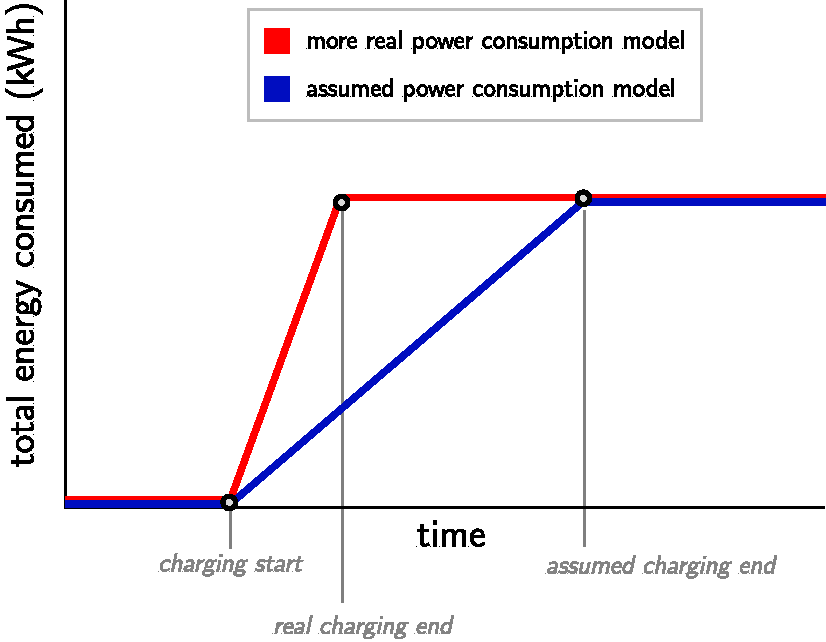
\includegraphics{charging-assumption.pdf}
    % \caption[Problem modelling overview]{Chapter content overview. }
\end{figure}

\section{Population numbers (ZSJ)}

\begin{figure}[hb]
    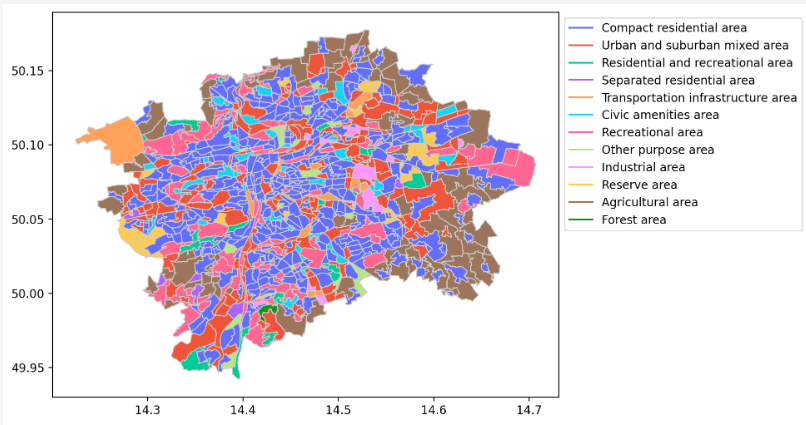
\includegraphics{zsj-type.png}
    % \caption[Problem modelling overview]{Chapter content overview. }
\end{figure}

\section{Points of Interest}


\section{People Mobility}

\begin{figure}[hb]
    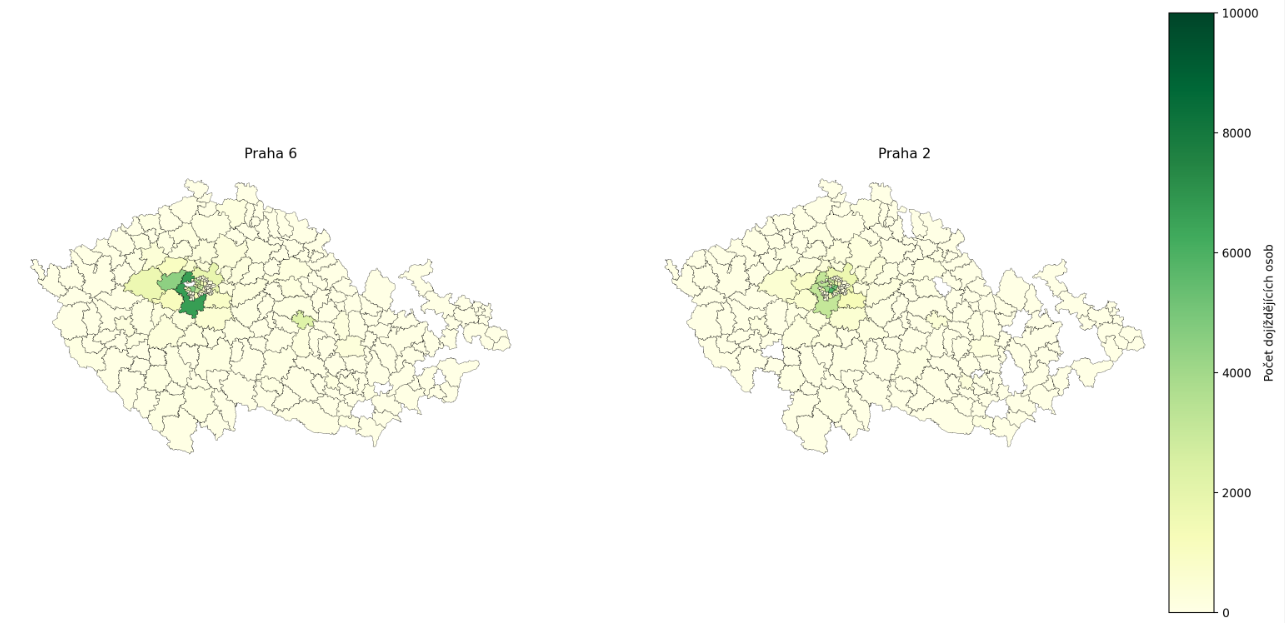
\includegraphics{commuting-people.png}
    \caption[Problem modelling overview]{Chapter content overview. }
\end{figure}

\section{Mobility Survey - cesko v pohybu}

\begin{figure}[hb]
    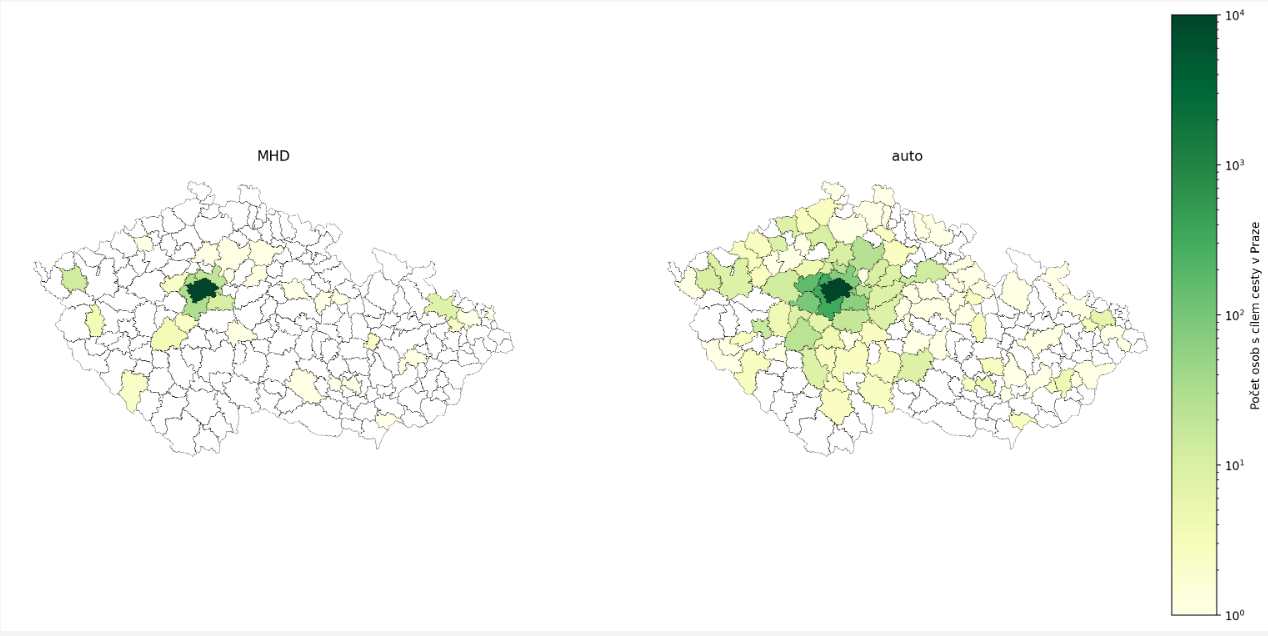
\includegraphics{vpohybu-trasnport-type.png}
    \caption[Problem modelling overview]{Chapter content overview. }
\end{figure}

---

Talks about what was extracted from datasets in \ref{ch:data}

\section{Spatial data}

\subsection{ZSJ Type and Population}

\subsection{Points of Interest}

Has statistically significant results for certain PoI \cite{hechtGlobalElectricVehicle2024}\cite{dongElectricVehicleCharging2019}
(\cite{dongElectricVehicleCharging2019} uses Gaussian cox model, \cite{hechtGlobalElectricVehicle2024} uses Neural networks and linear regression)

\cite{hechtGlobalElectricVehicle2024} states that radius of relevant PoIs is 2000metres. The research stated that the distance is sensible.
One solution is to just count all the PoIs in the radius but as they are more far away from the CP their relevance might decrease. The \cite{hechtGlobalElectricVehicle2024} thus uses importance factor for pair of PoI and CP.

$IF(PoI_i, CP_k) = max(r-d_{\text{sphere}}(PoI_i, CP_k),0)$


\subsubsection{Buildings (OsmPoisPbf)}


\subsubsection{Public Ammenities (OSMOX)}

how osmox works
\begin{figure}[hb]
    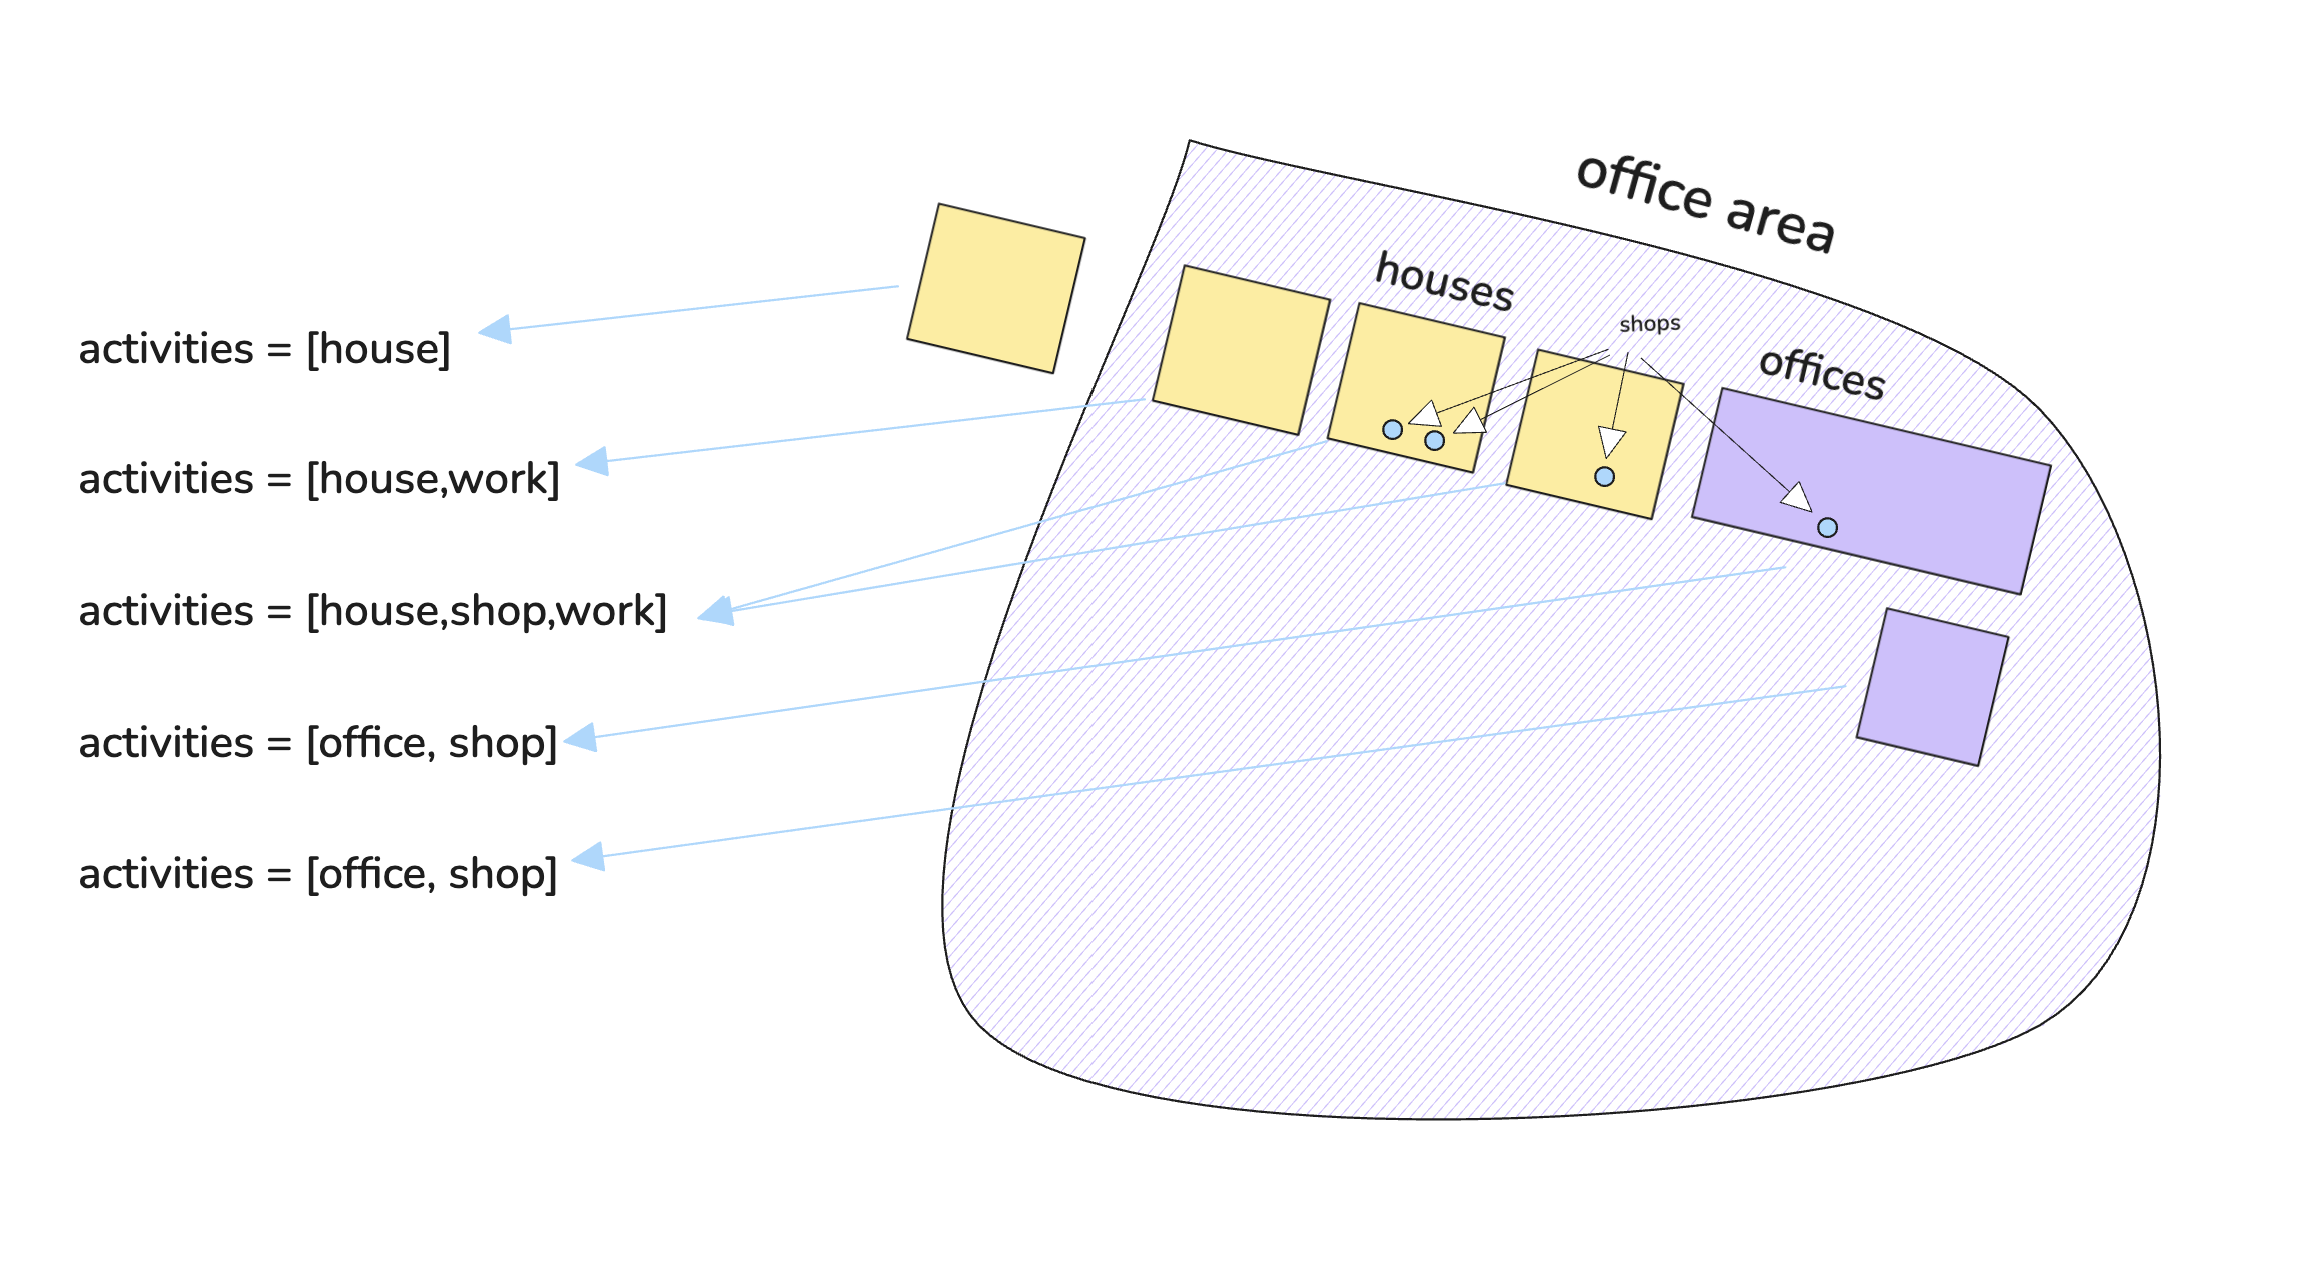
\includegraphics[width=0.7\textwidth]{osmox-poi.png}
    \caption[osmox]{osmox}
    \label{fig:nn-latent}
\end{figure}


\section{Charging profiles}


\begin{figure}[hb]
    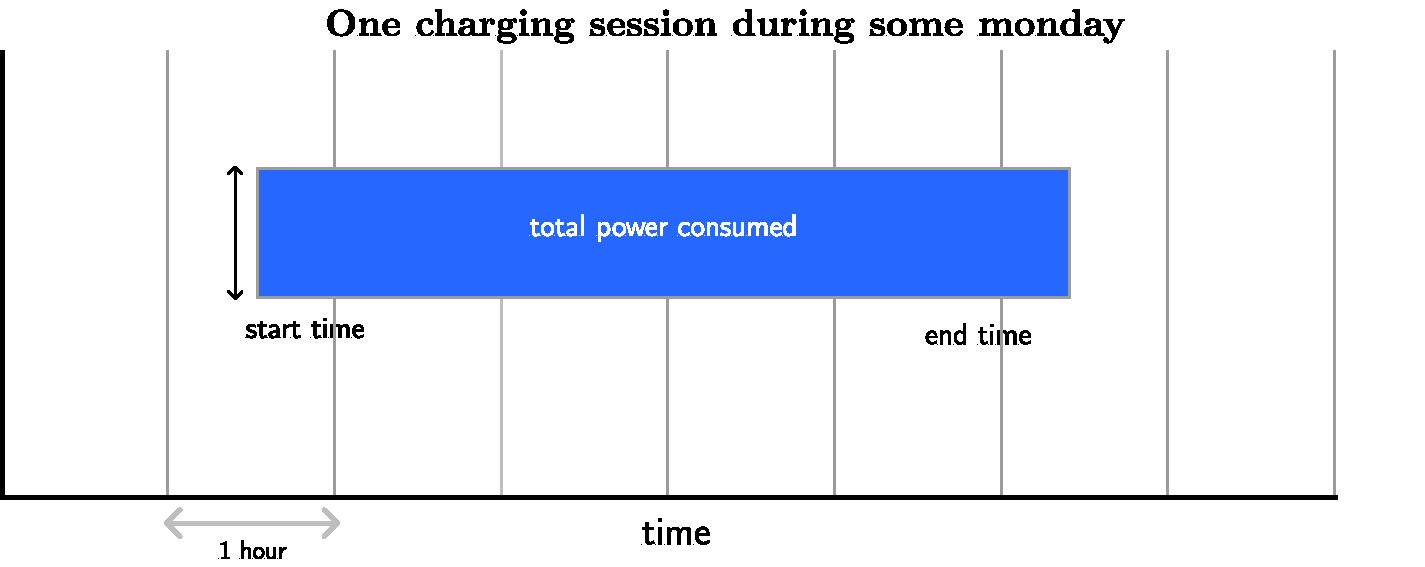
\includegraphics[width=0.7\textwidth]{cutting-1.pdf}
    % \caption[Cutting]{Cutting}
\end{figure}

\begin{figure}[hb]
    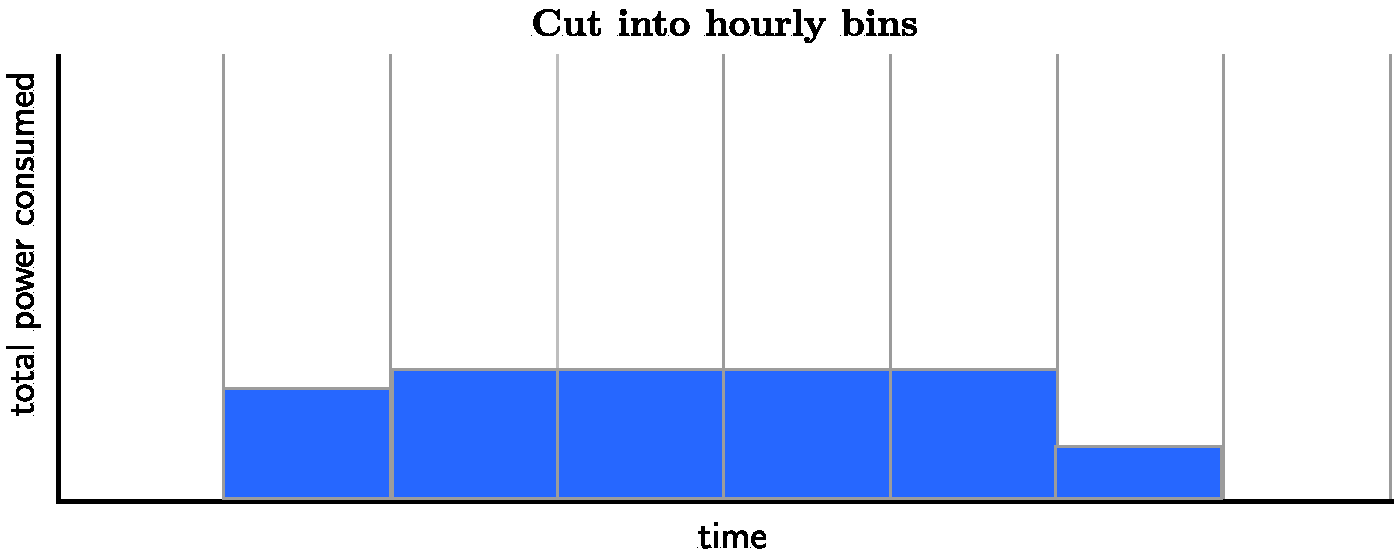
\includegraphics[width=0.7\textwidth]{cutting-2.pdf}
    % \caption[Cutting]{Cutting}
\end{figure}


\section{}
\pagelayout{margin}
\setchapterstyle{kao}
\setchapterpreamble[u]{\margintoc}
\chapter{Research and implementation}
\label{ch:problem}

\begin{figure}[hb]
    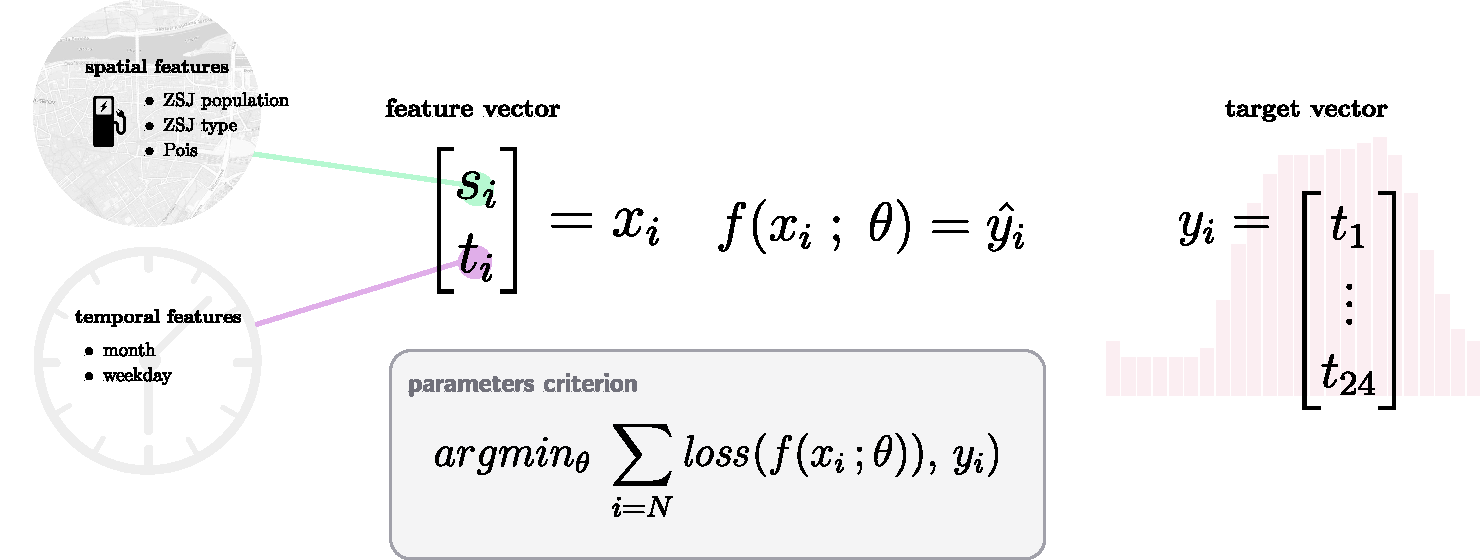
\includegraphics[width=1\textwidth]{diagram-detail}
    \caption[Problem modelling overview]{Problem approach overview}
\end{figure}

In this chapter, the problem will be formulated, and then an approach of solving it will be presented. The choice for the ML model will be discussed as well as its interpretable structure. A way of processing the data, splitting it into training and validation sets will be presented. And then a way to evaluate the model in comparison to other ML models will be described.

\section{Problem statement}

% \begin{marginfigure}
%     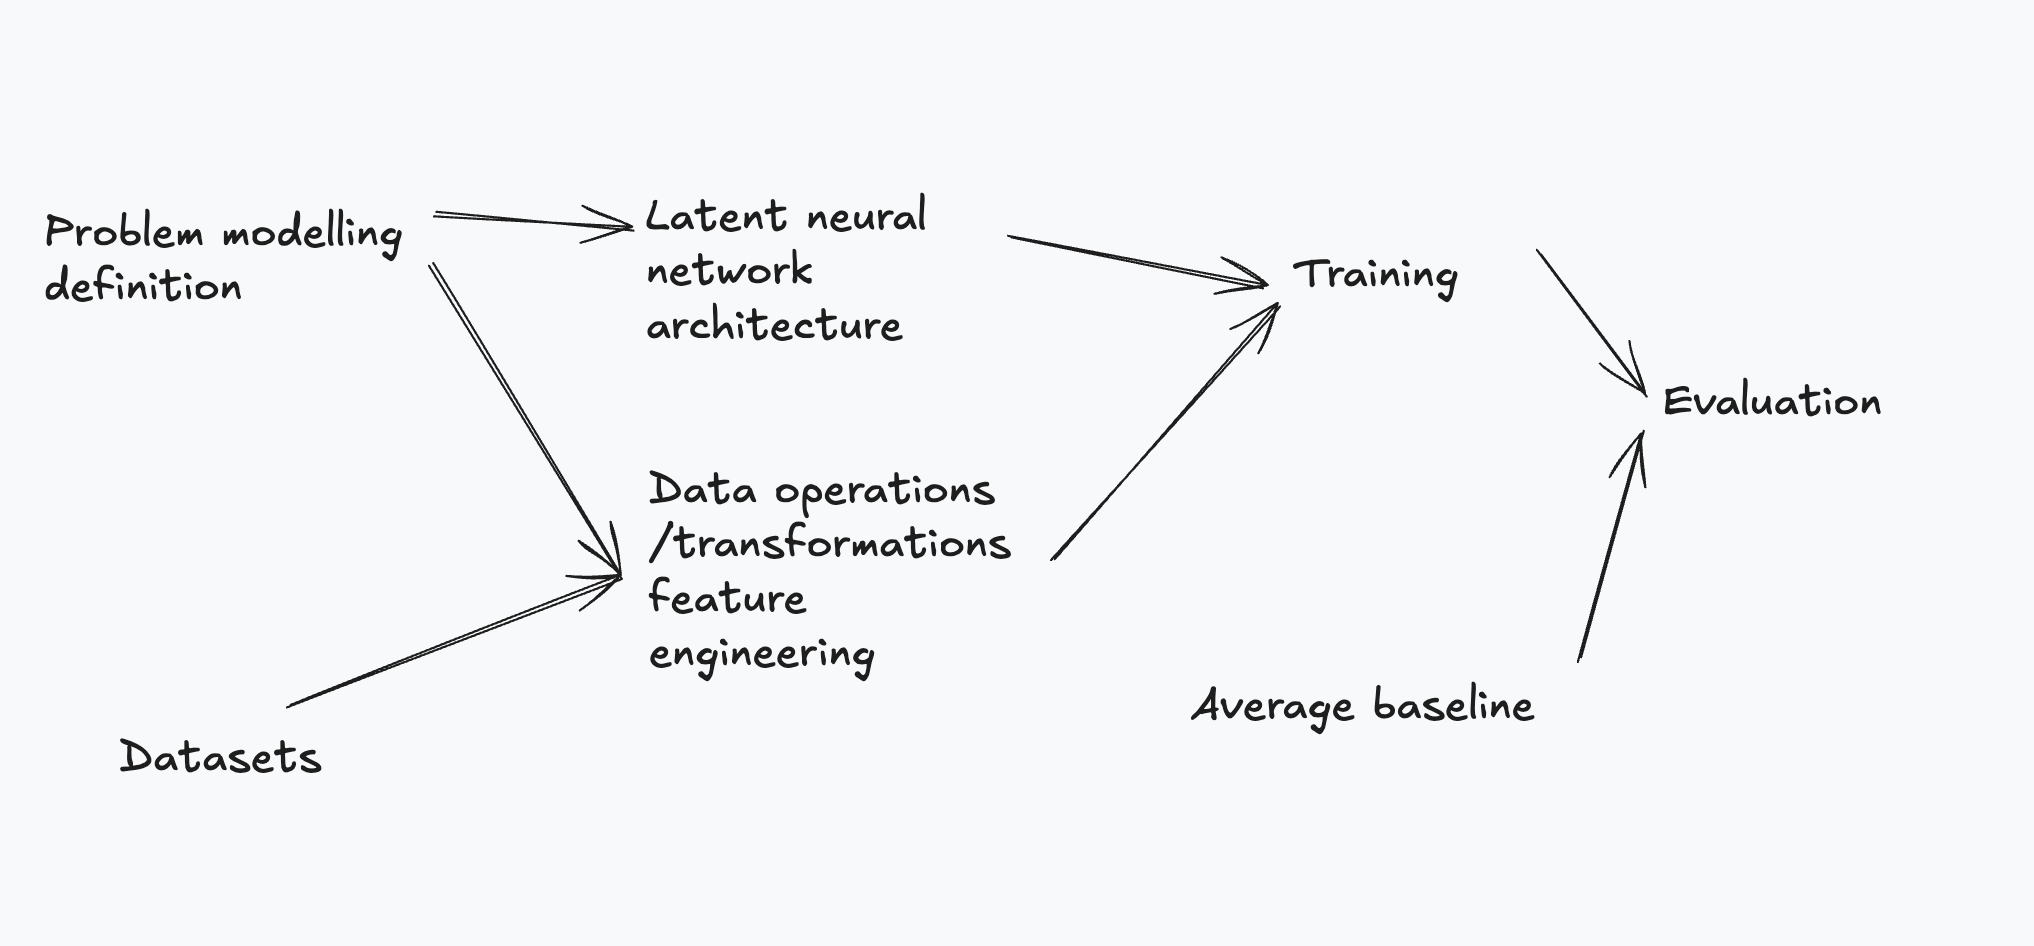
\includegraphics{diagram}
%     \caption[Problem modelling overview]{Chapter content overview.}
% \end{marginfigure}


We will be interested in estimating \acrfull{APC} from some set of features. And will like to know if our data-driven approach is viable.

To formulate how the model will look like, the model $f_\theta$ will execute the following mapping:

\[
    f_{\theta}: X \rightarrow Y
\]

Where $X$ will be the set of all feature vectors and $Y$ will be the set of all targets. The available data are split into \textit{training} \textit{test} and \textit{validation} sets. The first available at training time with goal of the training algorithm to minimize the empirical risk. How those sets are constructed is explained in \ref{sec:dataset-split}


$X \in \mathbb{R}^M$ and $Y\in \mathbb{R}^{24}$. And $| A | = | B | = P$.

The model function $f$ will have trainable parameters $\theta$. And we will be interested in finding such $\theta$ that minimizes the empirical risk:

\begin{equation}
    \mathit{loss_{total}}(f,\theta) = \frac{1}{P} \sum_{(x,y)\in\mathcal{T}} \alpha \cdot a_x + \beta \cdot b_x
\end{equation}

Where:

\begin{equation}
    \begin{split}
        a_x & = \mathit{loss_{power}}
        (\left \lVert f(x_i;\theta) \right \rVert_{1}, \left \lVert y_i \right \rVert_{1}) \\
        b_y & = \mathit{loss_{norm}}
        (\frac{f(x_i;\theta)}{\left \lVert f(x_i;\theta) \right \rVert_{1}}, \frac{y_i}{\left \lVert y_i \right \rVert_{1}})
    \end{split}
\end{equation}


where $\mathit{loss_{power}}$ and $\mathit{loss_{norm}}$ will be individual loss functions. Because we will be interested in model performance in estimating \acrfull{TDPC} and \acrfull{NDPC}. This will match with the chosen NN model architecture that will be discussed further in this chapter.

The use case of the model is to answer the EV charger planners' question: what will be the charger's power consumption if he decides to place a new \acrfull{CS} at a new place in Prague? And he is interested in its behavior given the temporal pattern\sidenote{e.g., how would a new charger at place $x$ perform on Thursdays of February}.

\section{Model features and feature engineering}

The feature vector of the model consist of \textbf{temporal} and \textbf{spatial} parts. Features regarding the charger's capabilities should be present as well, but that will be a limitation of the current chargers dataset that we will work with. The most useful will be the charger's maximum power output. Since that will most certainly influence the charger's average consumption. From this absence, the \acrfull{NDPC} will also be in our interest to estimate. Since the total power consumed might not have that big of an influence on it.

The feature items will fall into two categories divided by the data type. Either they will be categorical or numerical. If they will be categorical, they will be transformed with one-hot encoding. That is, given a category with $n$ items to transform the feature into $n$ binary features, where each binary feature will correspond to one of the possible values. For each observation, exactly one of these binary features will have the value 1, indicating the presence of that categorical value, while all others will be 0.

\marginnote{For example, if we have a categorical feature "day of week" with 7 possible values (Monday through Sunday), one-hot encoding transforms this into 7 binary features: "is\_Monday", "is\_Tuesday", etc. If an observation occurs on Wednesday, then the "is\_Wednesday" feature would be 1, while all other day features would be 0. This transformation allows the model to properly handle categorical variables without imposing an arbitrary ordinal relationship between category values.}

In our case, categorical features like the day of the week, month, and location characteristics will be one-hot encoded before being fed into the model. This will ensure that the model can effectively learn from these categorical variables without the constraints of numerical ordering.

Numerical features, on the other hand, will be standardized by subtracting the mean and dividing by the standard deviation to ensure all features will be on a comparable scale. This normalization process will prevent features with larger scales from dominating the learning process and will help achieve faster convergence during model training.

The feature vector will be constructed in the following way:

\begin{equation}
    \renewcommand*{\arraystretch}{1.5}
    x_i = \begin{bmatrix}
        s_i^T \\
        t_i^T
    \end{bmatrix}
\end{equation}

\textbf{spatial features} $s_i$ will be a vector of spatial features which contents will be described in \ref{tab:spatial-features-table} together with how this feature will be encoded.

\begin{equation}
    s_i = \begin{bmatrix}
        s_i^1  \\
        \vdots \\
        s_i^R
    \end{bmatrix}
\end{equation}

\begin{table*}[h!]
    \def\arraystretch{1.5}
    \caption{Overview of spatial features used in the feature vector. The additonal processing is describet at \ref{sec:spatial-transformations}}
    \label{tab:spatial-features-table}
    \begin{tabular}{p{1cm} p{3.5cm} p{1.8cm} p{3.5cm} p{4.5cm}}
        \toprule
        \textbf{Index} & \textbf{Name}                                                       & \textbf{Type} & \textbf{Value from}                  & \textbf{Additional processing}                                                                                             \\
        \midrule
        $s_{1}$        & ZSJ population                                                      & numeric       & charger in ZSJ polygon               & normalization by the polygon area                                                                                          \\
        $s_{2:10}$     & ZSJ type                                                            & categorical   & charger in ZSJ polygon               & one-hot encoding                                                                                                           \\
        $s_{11}$       & ZSJ number of addresses                                             & numeric       & charger in ZSJ polygon               & normalization by the polygon area                                                                                          \\
        $s_{12}$       & Number of people commuting into the district from inside Prague     & numeric       & charger in the district polygon      & normalization by the polygon area                                                                                          \\
        $s_{13}$       & Number of people commuting into the district from outside of Prague & numeric       & charger in the district polygon      & normalization by the polygon area                                                                                          \\
        $s_{14:162}$   & Points of Interest                                                  & numeric       & number of PoIs by euclidean distance & importance calculation (value of single PoI is 1 if its distance from charger is 0, 0 if it is of distance 2km or further) \\
        \bottomrule
    \end{tabular}
\end{table*}

\textbf{temporal features} $t_i$ will be a vector of temporal features which contents will be described in \ref{tab:temporal-features-table} together with how this feature will be encoded.

\begin{equation}
    t_i = \begin{bmatrix}
        t_i^1  \\
        \vdots \\
        t_i^P
    \end{bmatrix}
\end{equation}

\begin{table*}[h!]
    \caption{Overview of temporal pattern used in feature vector.}
    \label{tab:temporal-features-table}
    \begin{tabular}{p{1cm} p{3.5cm} p{1.8cm} p{3.5cm} p{4.5cm}}
        \toprule
        \textbf{Index} & \textbf{Name}   & \textbf{Type} & \textbf{Value from} & \textbf{Additional processing} \\
        \midrule
        $t_{1:7}$      & day of the week & categorical   & \acrfull{APC}       & one-hot encoding               \\
        $t_{8:19}$     & month           & categorical   & \acrfull{APC}       & one-hot encoding               \\
        \bottomrule
    \end{tabular}
\end{table*}

\section{Architecture of the Latent Neural Network}

The formulation of the machine learning problem provides us with ability of many solutions. Mainly from the class of nerual networks.

Neural networks are computational models. They consist of layers of interconnected nodes or "neurons" that process information. A typical neural network contains an input layer that receives data, one or more hidden layers that perform computations, and an output layer that produces the final result. Each connection between neurons has an associated weight that is adjusted during the training process. Information flows through the network via activation functions, which introduce non-linearity and allow the network to learn non-linear patterns. The training process involves feeding the network with labeled examples and using optimization algorithms, typically variants of gradient descent, to minimize a loss function by adjusting the weights. Backpropagation is the primary algorithm used to calculate gradients and update weights efficiently.


This leads us to the proposed neural network with latent profiles. Diagram of the network is visible at \ref{fig:nn-latent}. Before diving into the detailed network architecture a high level overview. The goal of the network is to construct for its internal use latent profile matrix $R$, $R \in \mathbb{R}^{24 \times K}$ for which it predicts how they should be mixed.

\newpage

The network utilizes the following layers:

\newcommand{\nnmodule}[3]{%
    \begin{marginfigure}[1cm]
        \centering
        \includegraphics[width=1.8cm]{#2}
    \end{marginfigure}
    \item \textbf{#1} \\
    #3
    \vspace{2mm}
}


\begin{itemize}
    \item[] \textbf{Trainable layers:}
          \begin{itemize}
              \nnmodule{Fully connected (Linear transformation)}{nn-modules/fully-conn.pdf}{%
                  $\text{Linear}^n_m(x) = W x + b$ \\
                  $\text{Linear}^n_m: \mathbb{R}^n \rightarrow \mathbb{R}^m \; , \;
                      W \in \mathbb{R}^{m \times n} \; , \;
                      b \in \mathbb{R}^m$ \\
                  $W, b$ are learnable \\

                  \vspace{2mm}

                  ...
              }

              \nnmodule{Latent vectors (Embedding)}{nn-modules/grad-parameter.pdf}{%
                  $\text{LatentVec}_K = R$ \\
                  $\text{LatentVec}_K: \emptyset \rightarrow \mathbb{R}^{24 \times K}$ \\
                  $R$ is learnable

                  \vspace{2mm}

                  ...
              }

          \end{itemize}

    \item[] \textbf{Non-parametric operations:}
          \begin{itemize}
              \nnmodule{Softplus (Smooth activation)}{nn-modules/softplus.pdf}{%
                  $f(x) = \ln(1 + e^x)$ \\
                  $f: \mathbb{R} \rightarrow \mathbb{R}^+$

                  \vspace{2mm}

                  ...
              }

              \nnmodule{Normalization}{nn-modules/norm.pdf}{%
                  $\text{Norm}(x) = \frac{x}{\|x\|_2}$ \\
                  $\text{Norm}: \mathbb{R}^n \rightarrow \{y \in \mathbb{R}^n : \|y\|_2 = 1\}$ \\
                  input dimension matches output dimension \\

                  \vspace{2mm}

                  ...
              }

              \nnmodule{Leaky-relu}{nn-modules/leaky-relu.pdf}{%
                  $\text{LReLU}(x) = \begin{cases}
                          x        & \text{if } x > 0    \\
                          \alpha x & \text{if } x \leq 0
                      \end{cases}$ \\
                  $\text{LReLU}: \mathbb{R} \rightarrow \mathbb{R} \; , \; \alpha \text{ is a hyperparameter}$ \\

                  \vspace{2mm}

                  Extension of ReLU. In this work there is no clear motivation for its use over tanh or ReLU.
              }
          \end{itemize}
\end{itemize}

\vspace{5mm}

\newpage

Those layers joined together form 3 modules. Each of which has assigned purpose by the way the are constructed and what is their possible output value range.

\begin{itemize}
    \item[] \textbf{Non-parametric operations:}
          \begin{itemize}
              \nnmodule{f module (Latent profile probabilities)}{nn-modules/f-module.pdf}{%
                  $f: \mathbb{R}^d \rightarrow \mathbb{R}^K$ \\
                  $f = \text{Softmax} \circ \text{Linear}_{K} \circ \text{LeakyReLU} \circ \text{Linear}_{64} \circ \text{LeakyReLU} \circ \text{Linear}_{h}$ \\
                  Where $d$ is feature size, $h$ is hidden size, and $K$ is latent profiles count \\
                  Outputs normalized weights for latent profiles

                  \vspace{3mm}

                  Purpose of this module is to predict the contribution of individual profiles into the resulting output normalized profile. In other words, this module is tasked with estimating the day rhythm of the charger without the actual total power. The input is feature vector, and it is transformed by two linear layers and ReLUs. The output is  vector of $K$ values and is transformed by softmax to ensure the sum of its values equals 1.
              }

              \nnmodule{g module (Total power)}{nn-modules/g-module.pdf}{%
                  $g: \mathbb{R}^d \rightarrow \mathbb{R}$ \\
                  $g = \text{Linear}_{1} \circ \text{LeakyReLU} \circ \text{Linear}_{32} \circ \text{LeakyReLU} \circ \text{Linear}_{h_g}$ \\
                  Where $d$ is feature size and $h_g$ is hidden size for g module

                  \vspace{3mm}

                  This module predicts just the total power for the given temporal pattern and location. It consists of 3 linear layers joined with LReLU. Its input is a feature vector and outputs just one scalar. With which combined output of $h$ and $f$ is multiplied at the end to obtain the prediction.
              }

              \nnmodule{h module (Latent profiles)}{nn-modules/h-module.pdf}{%
                  $h(\mathbf{x}) = f(\mathbf{x}) \cdot R^T$ \\
                  $p: \mathbb{R}^d \rightarrow \mathbb{R}^T$ \\
                  Where $R \in \mathbb{R}^{T \times K}$ is the normalized latent profiles matrix \\
                  $T$ is time granularity (24), $K$ is latent profiles count

                  \vspace{3mm}

                  \lipsum[3]
              }
          \end{itemize}
\end{itemize}

\vspace{5mm}

\newpage

Outputs of h and f modules are then combined like so:

\begin{equation}
    \begin{split}
         & \text{Combine}(R,p) = \sum_{i=1}^K p_i \, R_i                                             \\
         & \text{Combine}: \mathbb{R}^{24 \times K} \times \mathbb{R}^K \rightarrow \mathbb{R}^{24}÷
    \end{split}
\end{equation}

This is then multiplied by the scalar from g module which finally gives us the resulting prediction.

\begin{figure}[hb]
    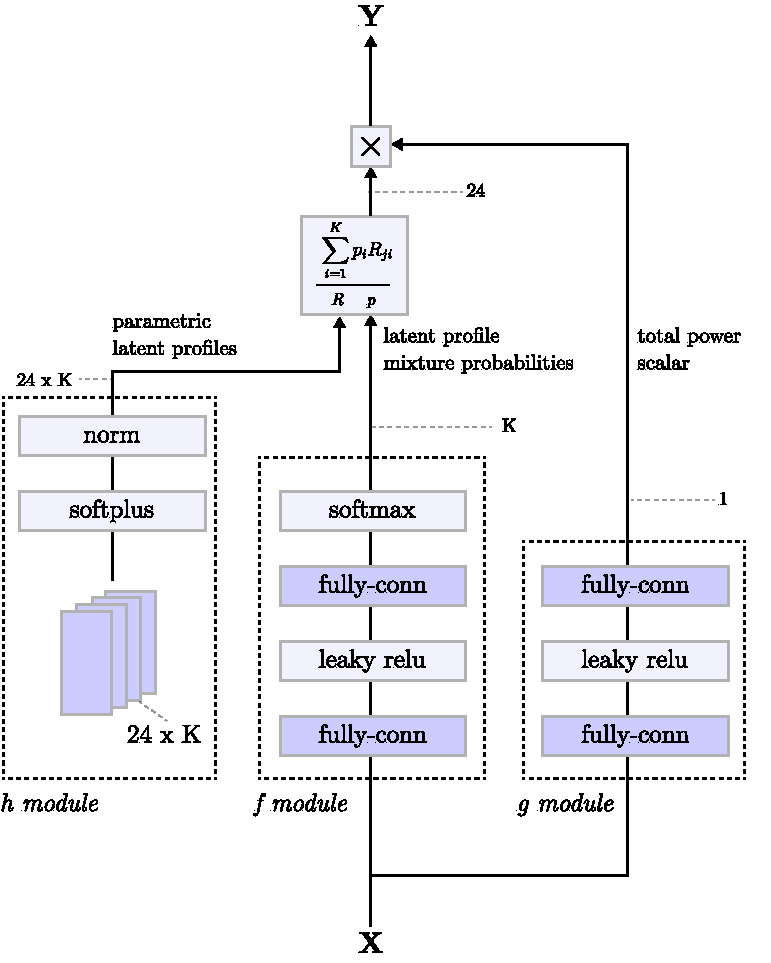
\includegraphics[width=0.8\textwidth]{nn-latent-architecture.pdf}
    \caption[Latent Neural Network Architecture]{Latent neural network architecture. Light blue rectangles denote NN layers without trainable parameters. While blue denotes layers with parameters learned by SGD. Notation borrowed from Fleurets book "Little book of deep learning"}
    \label{fig:nn-latent}
\end{figure}

The model is implemented in Python with use of Pytorch library \sidecite{paszke2019pytorchimperativestylehighperformance}.

\newpage


\section{Dataset splitting}
\label{sec:dataset-split}

To elaborate more on the way the datasets $\mathcal{T},\mathcal{S},\mathcal{V}$  are split. Since we are interested in modelling demand for location. We cannot just take all the \acrlong{APC}. Because of an issue, where one location has multiple \acrshort{ABM} for various \acrlong{TP} and also because the \acrshort{CS} has multiple \acrshort{CP}. And there might be a high correlation between the multiple \acrshort{CP} and our goal is for the model to be able to estimate demand for new locations. So the split is done based on location. Where features for each location can be only present in one of the sets.

% \begin{equation}
%     \begin{split}
%         \textit{train}:      \; \mathcal{T} & = ((x_i, y_i) \in X \times Y |\, i = 1,\dots, P) \\
%         \textit{test}:       \; \mathcal{S} & = ((x_i, y_i) \in X \times Y |\, i = 1,\dots, R) \\
%         \textit{validation}: \; \mathcal{V} & = ((x_i, y_i) \in X \times Y |\, i = 1,\dots, O)
%     \end{split}
% \end{equation}


\begin{itemize}
    \item \textbf{Train} dataset is used for training the model with use of \acrlong{SGD} for empirical risk minimization.
          \begin{equation}
              \label{eq:train}
              \textit{train}: \; \mathcal{T} = ((x_i, y_i) \in X \times Y |\, i = 1,\dots, P)
          \end{equation}
          \vspace{3mm}


    \item \textbf{Test} dataset is used for inspecting results of the model to see its performance on never seen data and tuning hyperparameters. And is used as an estimate of true model risk.

          \begin{equation}
              \label{eq:test}
              \textit{test}:       \; \mathcal{S}  = ((x_i, y_i) \in X \times Y |\, i = 1,\dots, R)
          \end{equation}
          \vspace{3mm}
    \item \textbf{Validation} dataset is used to obtain the final model risk on model with already trained parameters and chosen hyperparameters.
          \begin{equation}
              \label{eq:validation}
              \textit{validation}: \; \mathcal{V} = ((x_i, y_i) \in X \times Y |\, i = 1,\dots, O)
          \end{equation}
\end{itemize}

\section{Training procedure}

To train the model, we utilize the traditional Pytorch training procedure.
It was conducted using mini-batching \acrfull{SGD} optimization. The model was trained iteratively over several epochs with early stopping to prevent overfitting.

The batch size was selected to be X\todo{insert value} and the model took Y \todo{insert value} epochs with early termination before starting to overfit the training dataset.



\section{Other models for quantitative comparison}

The model is quantitatively compared with other models from the filed of machine learning. Results from the comparsion can motivate further research with the existing model or enable to quickly reject it.

One issue arrises from our custom loss, which is a mix with of two $L1$ losses. The ML models assume they want to minimize L1 loss. This might seem naive and not as a direct comparison hovewer more info will be provided in \ref{ch:results}.

The models for comparsion are the following:

\begin{itemize}
    \item \textbf{Average} - The most simple baseline. That is taking average over the whole datasets feature vectors and using that value as a prediction. Both the train and test datasets $\mathcal{T},\mathcal{S},$ are utilized for this "model". It does not take into account the input and utilizes one value for any further predictions.

          We provide the implementation.
          \begin{equation}
              \begin{split}
                   & f(z)^{\mathcal{D}}  = \frac{1}{|\mathcal{D}|} \sum_{(x,\_) \in \mathcal{D}} x \\
                   & f: \mathbb{R}^m \rightarrow \mathbb{R}^n                                      \\
                   & n,m \in \mathbb{N}, \mathcal{D} \in  (X \times Y)^p, p \in \mathbb{N}
              \end{split}
          \end{equation}


    \item \textbf{Linear regression} - Linear model

          Implementation is taken from Python library Scikit Learn \sidecite{scikit-learn}
          \begin{equation}
              \begin{split}
                   & f(z) = \alpha  + \beta z                                   \\
                   & f: \mathbb{R}^m \rightarrow \mathbb{R}^n                   \\
                   & \alpha \in \mathbb{R}^{n \times m}, \beta \in \mathbb{R}^n
              \end{split}
          \end{equation}
    \item \textbf{XGBoost} - A scalable end-to-end tree boosting system \sidecite{Chen_2016}
\end{itemize}

The peformance of these models is compared with our model based on mean absolute error, mean square error on the following: \acrlong{APC}, \acrlong{TDPC} and \acrlong{NDPC}.

In case of the profiles. We divide the loss by 24. To obtain error for an hour instead of the 24 hours.

\setchapterstyle{kao}
\setchapterpreamble[u]{\margintoc}

\setchapterstyle{kao}
\setchapterpreamble[u]{\margintoc}
\chapter{Results}
\label{ch:results}

\todo{Say that the other ml models do not need more detailed loss functions since our model was not convincingly better}


In this chapter. Prediction model results will be discussed. An quantitative comparison to other models is provided.

To evaulate the quality of the model and its potential benefits.

\section{Quantitative comparison to other models}
\label{sec:res-comparison}

% Please add the following required packages to your document preamble:

\begin{table*}[h!]
    \caption{Comparison of model performance metrics including Mean Absolute Error (MAE) and Mean Squared Error (MSE) with their normalized and power variants.}
    \label{tab:my-table}
    \begin{tabular}{p{3.3cm} p{1.5cm} p{1.8cm} p{2.2cm} p{1.5cm} p{1.8cm} p{2.2cm}}
        \toprule
        \textbf{Model}         & \textbf{MAE} & \textbf{MAE norm} & \textbf{MAE power} & \textbf{MSE} & \textbf{MSE norm} & \textbf{MSE power} \\
        \midrule
        ChargingProfileModel   & 86.3404      & 0.0447            & 1553.9763          & 33729.4410   & 0.0057            & 7748441.2767       \\
        LinearRegression       & 107.9335     & 0.0962            & 2181.7242          & 41590.8896   & 2.9124            & 10658337.9148      \\
        TrainAverageModel      & 87.9659      & 0.0435            & 1629.9461          & 33973.4273   & 0.0057            & 7853195.2634       \\
        ValidationAverageModel & 87.9659      & 0.0435            & 1629.9461          & 33973.4273   & 0.0057            & 7853195.2634       \\
        XGBoost                & 92.4132      & 0.0456            & 1639.3703          & 42282.8242   & 0.0065            & 7993035.6818       \\
        \bottomrule
    \end{tabular}
\end{table*}
\section{Qualitative latent profiles analysis}

\textit{Inspection of the outputed latent profiles in prague together with hypotethising if that at least makes sense. Show the latent profile contribution on the training dataset because it interesting to see what it learned from the data and not necesarily rating its prediction power.}

\section{Tool for visualisation of prediction results}
To be able to inspect the prediction results in spatial context a tool was also developed with use of Streamlit\sidecite{StreamlitFasterWay2021}. The dashboard is in a form of a webapplication.
It consists of two screens.
First one allows inspection of overall model losses as visible in \ref{sec:res-comparison}. In bar charts and tabular formats. Where the bar chart shows all the types of losses relatively to each other.
\begin{figure}
    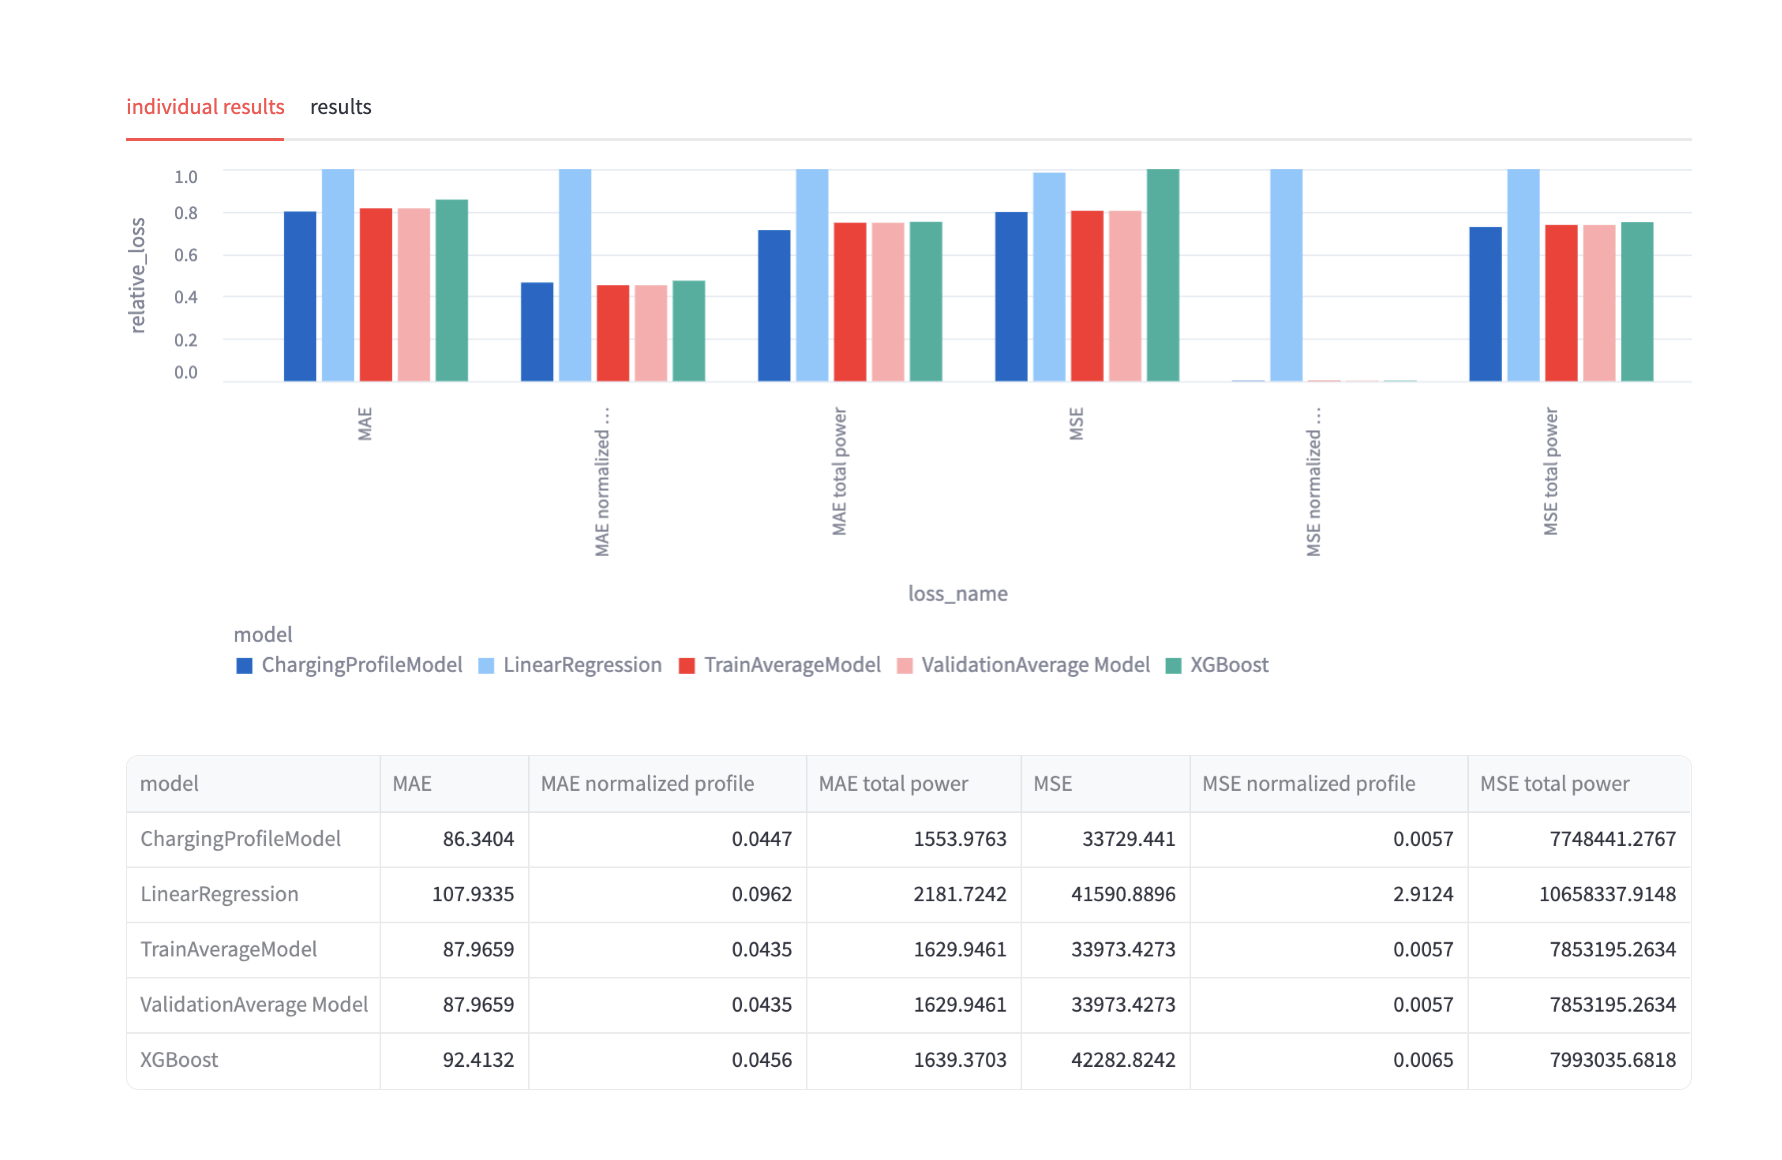
\includegraphics{data-dashboard-losses.png}
    \caption[]{Data dashboard website showing bar chart with relative losses of the models}
    \labfig{dasboard-all}
\end{figure}

The second screen displays table of all charging location together with day of the week and month. The individual rows of the table are selectable. When selection haapens location of the charger in map is shown and prediction from the model together with other models used for comparison is computed and its results are shown in a bar chart graph. Together with losses agains the original label $y$ value.

\begin{figure}
    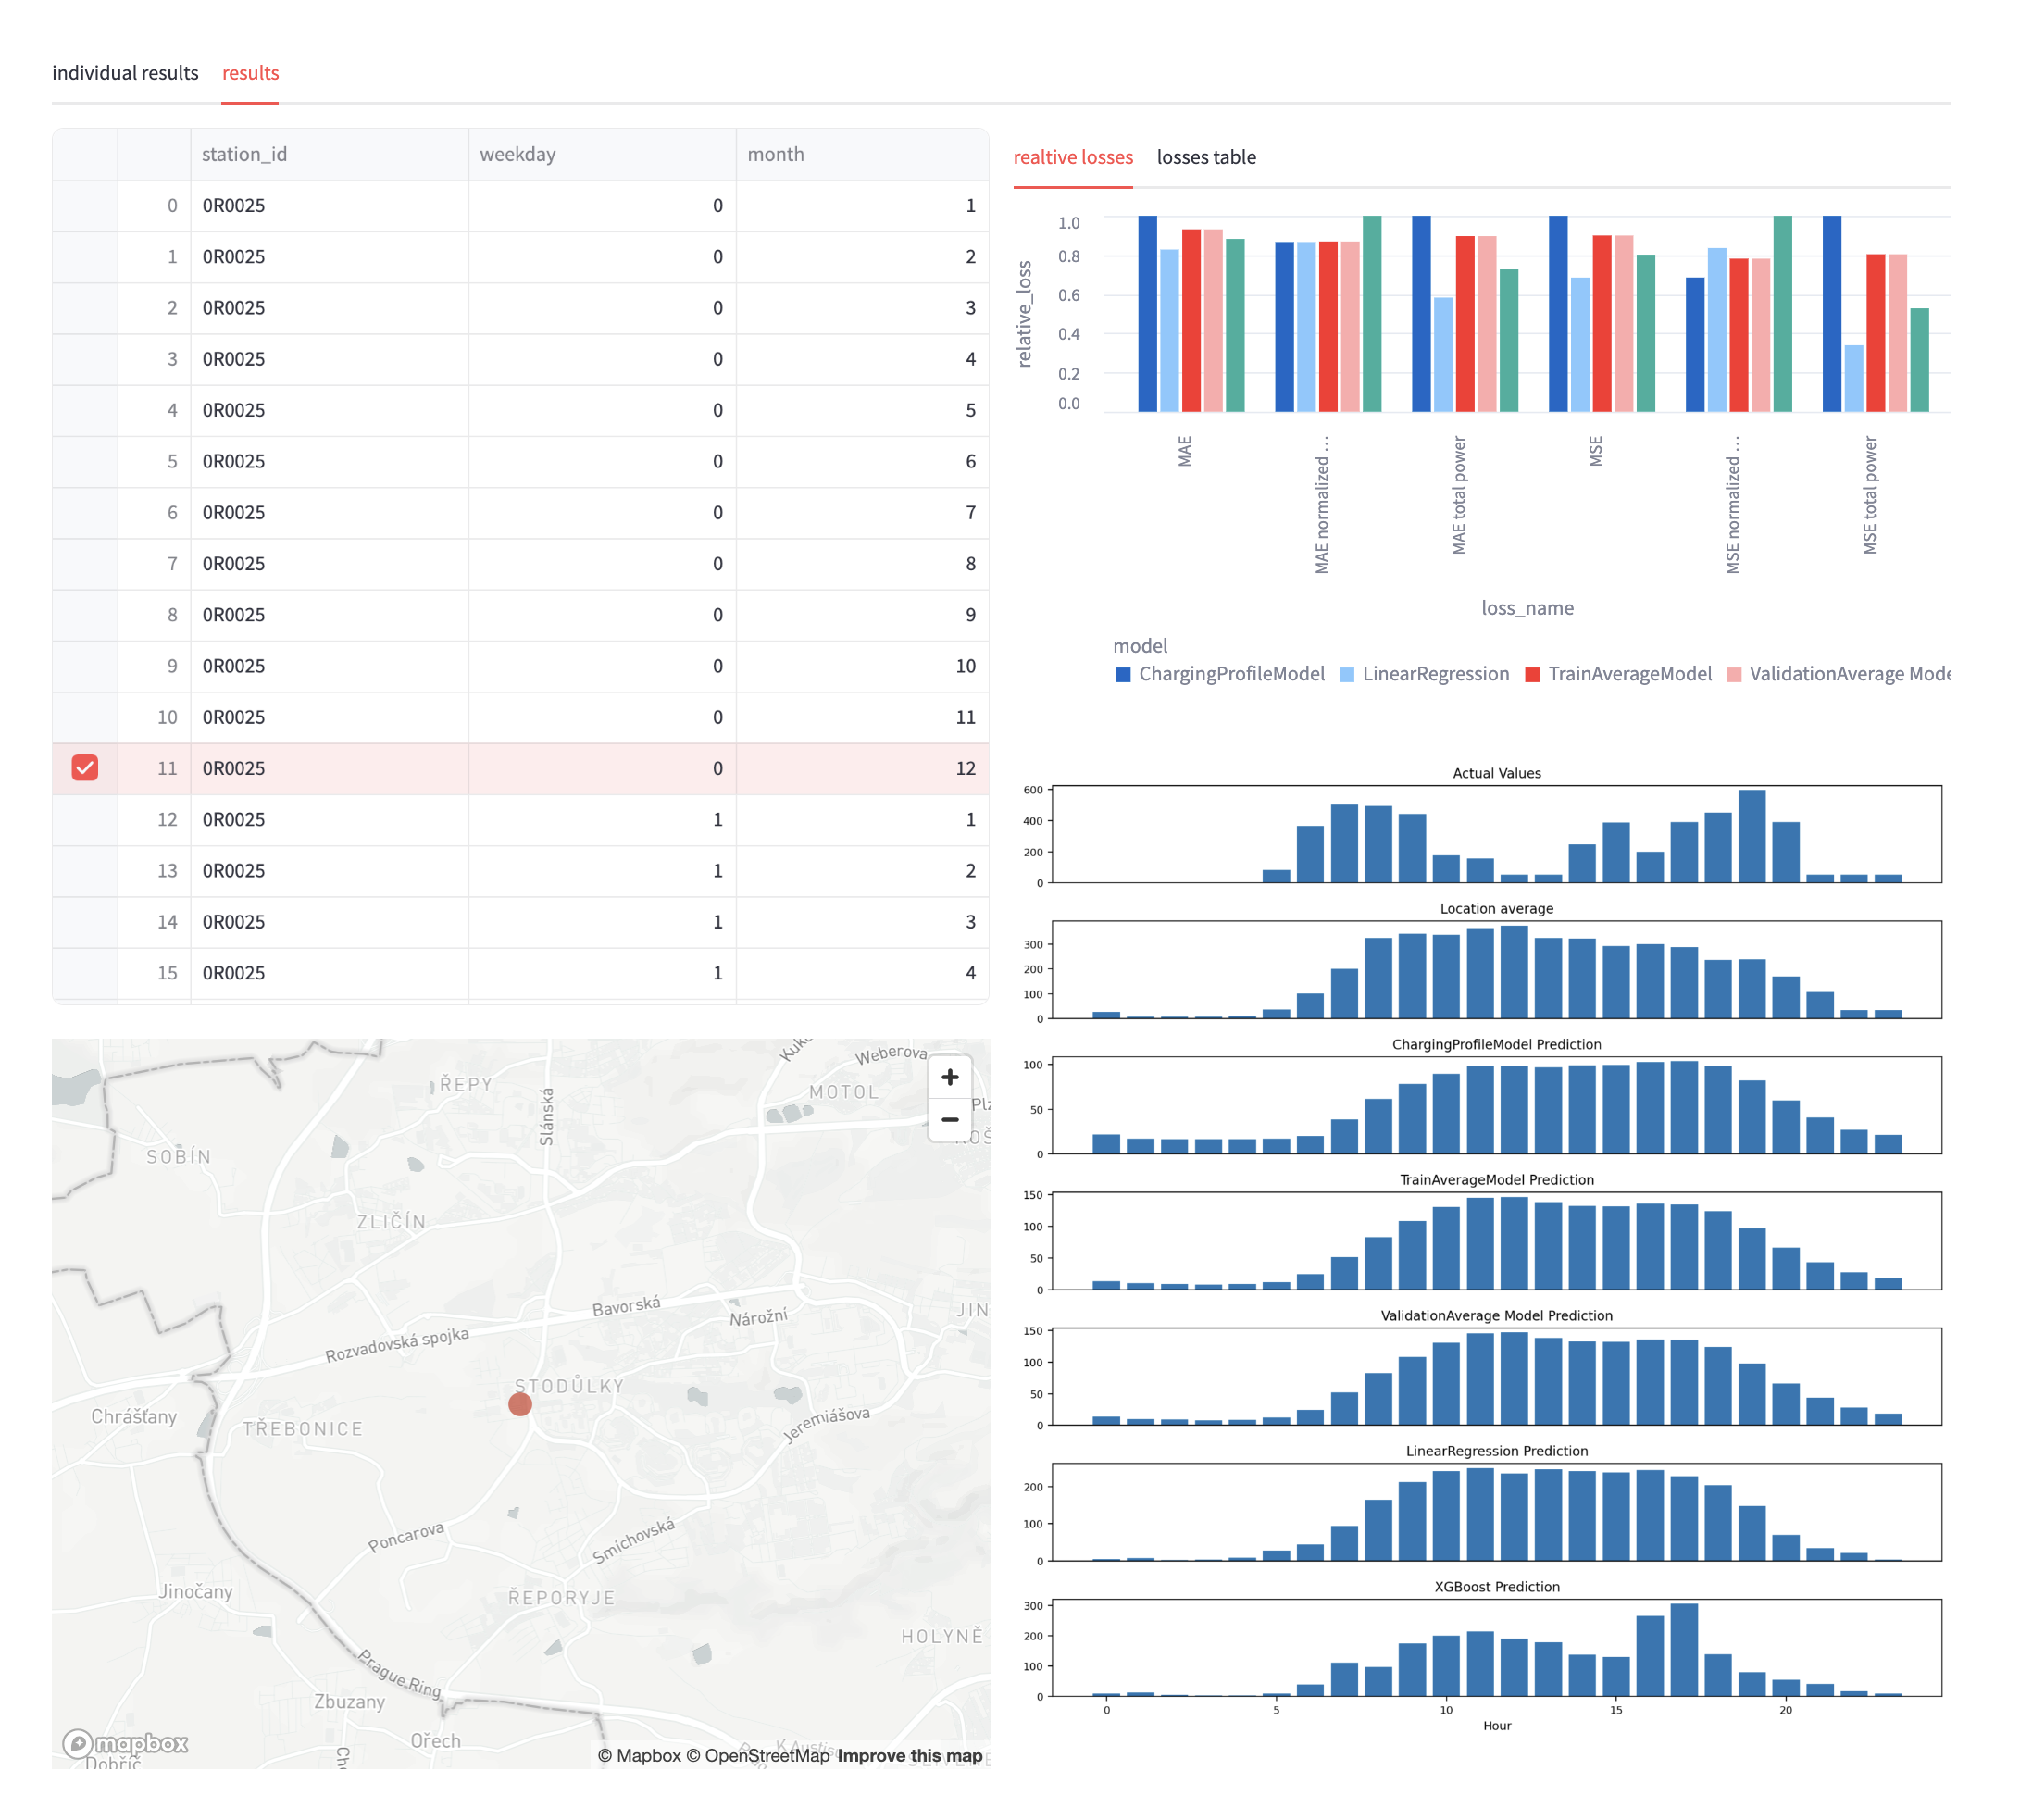
\includegraphics{data-dashboard-individual-predictions.png}
    \caption[]{Data dashboard website showing table with data from validation data set with one selected row. Of which the prediction is computed from the main model and the other models for comparison.}
    \labfig{dasboard-individual}
\end{figure}

\chapter{Conclusion}

How good we think we have been. And what did this work provide.

\textit{what was achieved in regards of the beginning goals}

\section{Future work}

What to do next to improve the model. What datases to be included.


\appendix % From here onwards, chapters are numbered with letters, as is the appendix convention


\backmatter % Denotes the end of the main document content
\setchapterstyle{plain} % Output plain chapters from this point onwards

%----------------------------------------------------------------------------------------
%	BIBLIOGRAPHY
%----------------------------------------------------------------------------------------

% The bibliography needs to be compiled with biber using your LaTeX editor, or on the command line with 'biber main' from the template directory


\begingroup % Local scope for the following commands

% Define the style for the TOC, LOF, and LOT
%\setstretch{1} % Uncomment to modify line spacing in the ToC
%\hypersetup{linkcolor=blue} % Uncomment to set the colour of links in the ToC
\setlength{\textheight}{230\hscale} % Manually adjust the height of the ToC pages

% Turn on compatibility mode for the etoc package
\etocstandarddisplaystyle % "toc display" as if etoc was not loaded
\etocstandardlines % "toc lines" as if etoc was not loaded

\listoffigures % Output the list of figures

% Comment both of the following lines to have the LOF and the LOT on different pages
\let\cleardoublepage\bigskip
\let\clearpage\bigskip

\listoftables % Output the list of tables

\endgroup

\defbibnote{bibnote}{Here are the references in citation order.\par\bigskip} % Prepend this text to the bibliography
\printbibliography[heading=bibintoc, title=Bibliography, prenote=bibnote] % Add the bibliography heading to the ToC, set the title of the bibliography and output the bibliography note

\renewcommand{\nomname}{Notation} % Rename the default 'Nomenclature'
\renewcommand{\nompreamble}{The next list describes several symbols that will be later used within the body of the document.} % Prepend this text to the nomenclature

\printnomenclature % Output the nomenclature

%----------------------------------------------------------------------------------------
%	GLOSSARY
%----------------------------------------------------------------------------------------

% The glossary needs to be compiled on the command line with 'makeglossaries main' from the template directory

\setglossarystyle{listgroup} % Set the style of the glossary (see https://en.wikibooks.org/wiki/LaTeX/Glossary for a reference)
\printglossary[title=Special Terms, toctitle=List of Terms] % Output the glossary, 'title' is the chapter heading for the glossary, toctitle is the table of contents heading

%----------------------------------------------------------------------------------------
%	INDEX
%----------------------------------------------------------------------------------------

% The index needs to be compiled on the command line with 'makeindex main' from the template directory

% \printindex % Output the index

%----------------------------------------------------------------------------------------
%	BACK COVER
%----------------------------------------------------------------------------------------

% If you have a PDF/image file that you want to use as a back cover, uncomment the following lines

%\clearpage
%\thispagestyle{empty}
%\null%
%\clearpage
%\includepdf{cover-back.pdf}

%----------------------------------------------------------------------------------------

\end{document}
